\documentclass[a4paper, 12pt]{article}
\usepackage[hidelinks]{hyperref} 
%\usepackage{apacite}
\usepackage[margin=1.1in]{geometry}
\usepackage{titling}
\usepackage{amsmath}
\usepackage{amssymb} %math symbol library
\usepackage{graphicx}
\setcounter{secnumdepth}{3}
\usepackage{setspace}
\usepackage{pslatex} %Times font
\usepackage{titletoc}
\usepackage{tocloft}
\usepackage{soul}
\usepackage{multirow}
\usepackage{hhline}
\usepackage{array}
\usepackage{pdfpages}
\usepackage[]{appendix}
%\usepackage{longtable}
%\usepackage{wrapfig}

\usepackage[font=small,it]{caption}
%\usepackage{subfig}
%\usepackage{tabularx}
%\usepackage{setspace}
\usepackage[none]{hyphenat} %No breaking hyphenation
%\renewcommand{\thesection}{\Roman{section}}  %no numbering but in TOC


\newcommand{\subtitle}[1]{
	\posttitle{
		\par\end{center}
		\begin{center}\large#1\end{center}
		\vskip0.5em}
}
%
%

%\doublespacing
\renewcommand\thesubsubsection{\thesubsection.\Alph{subsubsection}}

\begin{document}


%%Title page/ cover page  ================================
\begin{titlepage}

\title{\huge{ELEC 481\\ \large{Linear Systems \vspace{5ex}}}}
	\subtitle{\large{Lab Report} \\  \large{}
	\vspace{15ex}}
	

\author{
Name: Yuan Sun  \hspace{15ex}  ID: 26465358  \\
Name: Youcheng Zheng  \hspace{8.5ex}  ID: 25879485  \\
Name: Shuixi Li \hspace{15.2ex}  ID: 26327338 \\
\hspace{0.1ex}
Name: Zhuang Liu	\hspace{13ex}  ID: 29723986 \vspace{18ex}}


\date{\today}

\clearpage
\maketitle                       %
\thispagestyle{empty}  % make title page no numbering
\end{titlepage}
\newpage


%% Table of content  ====================================

\tableofcontents
\titlecontents{section}
[0em]
{\filcenter\large\bfseries}
{\contentslabel{3ex}}
{}
{\titlerule*{$\cdot$} \contentspage}  
%\thispagestyle{empty}  
\clearpage        
\newpage

\listoffigures
\listoftables
%\thispagestyle{empty}  
\clearpage        
\newpage

\setcounter{page}{1}

%% start the content of the report ===============================Finished==========
\section{Input-output equations of the system}\label{Equations}
\hspace{2.5ex}The laboratory we chose is industrial emulator. We decide to use two different models to describe this industrial emulator. 

\subsection{Rigid body model}
First model we use is rigid body model which is shown in figure~\ref{rigidbody}. We define the input is $T_D$ and output is $\theta_2$.

\begin{figure}[!htbp]
\centering
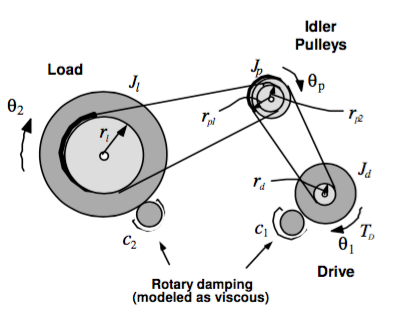
\includegraphics[scale = 0.7]{RigidBody}
\caption{Rigid Body model}
\label{rigidbody}
\end{figure}

For there are two disks, so two equations can be written. For $J_d$ is connected to idler pulley which is further connect to the $J_l$, the actual moment of inertia of drive disk $J_d^*$ is $J_d^* = J_d + J_p gr'^{-2} + J_lgr^{-2}$ where $gr = \dfrac{r_l r_{pl}}{r_{p2}r_d}$, $gr' = \dfrac{r_{p1}}{r_d}$. For the same reason, the actual moment of inertia of load disk $J_l^* = J_d gr^2 + J_p (gr/gr')^2 + J_l$. Therefore, the two equations associated with these two moment of inertia are: 

\begin{equation} \label{rigidbody1}
J_d^* \ddot{\theta}_1 + c_d^* \dot{\theta}_1 = T_d
\end{equation}

\begin{equation} \label{rigidbody2}
J_l^* \ddot{\theta}_2 + c_l^*\dot{\theta}_2 = gr T_d
\end{equation}
where $c_d^* = c_1 + c_2gr^{-2}$ and $c_l^* = c_1gr^2 + c_2$.

For equation~\ref{rigidbody2} relates $T_D$ to $\theta_2$, equation~\ref{rigidbody2} alone is enough to describe the system. 

Let $\mathbf{X} = \begin{bmatrix}
\theta_2	\\
\dot{\theta}_2	
\end{bmatrix}
$, 
$\mathbf{U} = \begin{bmatrix}
0 & T_D
\end{bmatrix}
$, the state equations are
\begin{equation} \label{rigidbodystate}
\mathbf{\dot{X}} = 
\begin{bmatrix}
\dot{\theta}_2 \\
\ddot{\theta}_2
\end{bmatrix} = 
%A
\begin{bmatrix}
0	&	1	\\
0	&	-\frac{c_l^*}{J_l^*}
\end{bmatrix} \mathbf{X} +
%B
\begin{bmatrix}
0\\
\frac{gr}{J_l^*}
\end{bmatrix} \mathbf{U}
\end{equation}
where $\mathbf{A} = \begin{bmatrix}
0	&	1	\\
0	&	-\frac{c_l^*}{J_l^*}
\end{bmatrix}$,
and $\mathbf{B} = \begin{bmatrix}
0\\
\frac{gr}{J_l^*}
\end{bmatrix}$.

The output equation is 
\begin{equation}
\mathbf{Y} = %C
\begin{bmatrix}
1	&	0
\end{bmatrix} \mathbf{X}
\end{equation}
where $\mathbf{C} =  \begin{bmatrix}
1	&	0
\end{bmatrix}$, and $\mathbf{D} = \begin{bmatrix} 0 \end{bmatrix}$.

\subsection{Flexible drive model}
To fully describe the system, we also use flexible drive model to analyze the industrial emulator shown in figure~\ref{flexible}. In the flexible drive model, the linear spring constant is taken into account. $T_D$ is considered as the input, and $\theta_2$ is considered as output. 


\begin{figure}[!htbp]
\centering
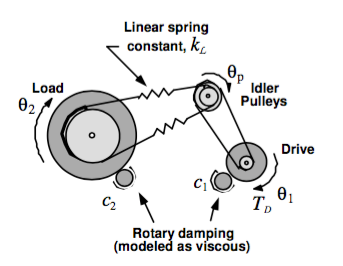
\includegraphics[scale = 0.7]{Dynamics}
\caption{Flexible drive model}
\label{flexible}
\end{figure}

So the two equations associated with two moment of inertia are:

\begin{equation} \label{flexible1}
J_d^* \ddot{\theta}_1 + c_1\dot{\theta}_1 + k(gr^{-2}\theta_1 - gr^{-1} \theta_2) = T_D
\end{equation}

\begin{equation} \label{flexible2}
J_l \ddot{\theta}_2 + c_2\dot{\theta}_2 + k(\theta_2 - gr^{-1}\theta_1) = 0
\end{equation}
where $k = 2k_L r_l^2$ and $J_d^* = J_d + gr'^2J_p$.

Let $\mathbf{X} = \begin{bmatrix}
\theta_1 	\\
\dot{\theta}_1	\\
\theta_2	\\
\dot{\theta}_2	
\end{bmatrix}
$, 
$\mathbf{U} = \begin{bmatrix}
0 & T_D	&	0	&	0
\end{bmatrix}
$, the state equations are
\begin{equation}\label{flexiblestate}
\mathbf{\dot{X}} = \begin{bmatrix}
\dot{\theta}_1	\\
\ddot{\theta}_1	\\
\dot{\theta}_2	\\
\ddot{\theta}_2	
\end{bmatrix}
 =  % A
 \begin{bmatrix}
 0	&	1	&	0	&	0	\\
 \frac{-kgr^{-2}}{J_d^*}	&	\frac{-c_1}{J_d^*}	&	\frac{kgr^{-1}}{J_d^*}	&	0	\\
 0	&	0	&	0	&	1	\\
 \frac{kgr^{-1}}{J_l}	&	0	&	\frac{-k}{J_l}	&	\frac{-c_2}{J_l}
 \end{bmatrix}
 \mathbf{X} + %B
 \begin{bmatrix}
 0	\\
 \frac{1}{J_d^*}	\\
 0	\\
 0
 \end{bmatrix} \mathbf{U}
\end{equation}
where $\mathbf{A} =  \begin{bmatrix}
 0	&	1	&	0	&	0	\\
 \frac{-kgr^{-2}}{J_d^*}	&	\frac{-c_1}{J_d^*}	&	\frac{kgr^{-1}}{J_d^*}	&	0	\\
 0	&	0	&	0	&	1	\\
 \frac{kgr^{-1}}{J_l}	&	0	&	\frac{-k}{J_l}	&	\frac{-c_2}{J_l}
 \end{bmatrix}$, 
 $\mathbf{B} =  \begin{bmatrix}
 0	\\
 \frac{1}{J_d^*}	\\
 0	\\
 0
 \end{bmatrix}$.

The output equation is
\begin{equation} \label{flexibleoutput}
\mathbf{Y} = \begin{bmatrix}
0	&	0	&	1	&	0	
\end{bmatrix} \mathbf{X}
\end{equation}
where $\mathbf{C} = \begin{bmatrix}
0	&	0	&	1	&	0	
\end{bmatrix} $, and $\mathbf{D} = \begin{bmatrix} 0 \end{bmatrix}$.

\vspace{7ex}
%% Find transfer function =====================Finished========================
\section{Find the transfer function of the open-loop system}
\subsection{Rigid body model}
\hspace{2.5ex}
The Laplace transform of equation~\ref{rigidbody1} and equation~\ref{rigidbody2} are:

\begin{equation}\label{laplacerigidbody1}
\dfrac{\theta_1 (s)}{T_D(s)} = \dfrac{1}{J_d^*s^2 + c_d^* s}
\end{equation}

\begin{equation} \label{laplacerigidbody2}
\dfrac{\theta_2 (s)}{T_D(s)} = \dfrac{gr}{J_l^* s^2 + c_l^*s} 
\end{equation}

\subsection{Flexible drive model}
The Laplace transform of equation~\ref{flexible1} and equation~\ref{flexible2} are:

\begin{equation} \label{laplaceflexible1}
\dfrac{\theta_1(s)}{T_D(s)} = \dfrac{J_l s^2 + c_2 s + k}{D(s)}
\end{equation}

\begin{equation} \label{laplaceflexible2}
\dfrac{\theta_2 (s)}{T_D (s)} = \dfrac{k/gr}{D(s)}
\end{equation}
where \begin{equation} \label{D(s)}
D(s) = J_d^*J_l s^4 +(J_d^*c_2 + J_lc_1) s^3 +(J_d^*k + J_lgr^{-2} k + c_1c_2) s^2 +(c_1k + c_2gr^{-2})s 
\end{equation}

\vspace{7ex}
%% obtain canonical forms===========================Finished==================
\section{Obtain the controllable, observable, and Jordan canonical forms}
%Rigid body model
\subsection{Rigid body model}
% Controllable
\subsubsection{Controllable canonical form}
\hspace{2.5ex}
Start with transfer function. 
\begin{equation}\label{rigidControllable}
\dfrac{\theta_2(s)}{T_D(s)} = \dfrac{gr}{J_l^*+ c_l^* s} = \dfrac{1}{s^2 + \frac{c_l^*}{J_l^*} s} \cdot \dfrac{gr}{J_l^*}
\end{equation}
where 
\begin{equation}
D_2(s) = s^2 + \frac{c_l^*}{J_l^*} s
\end{equation}

The system can be converted into the structure shown in figure~\ref{rigidControllableChart}. In other words, $\dfrac{Z(s)}{T_D(s)} = \dfrac{1}{D_2(s)} \longrightarrow D_2(s) Z(s) = T_D$. 


\begin{figure}[!htbp]
\centering
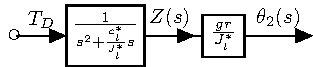
\includegraphics[scale = 1.5]{Controllable4RigidBody}
\caption{State diagram for controllable canonical form of rigid body model}
\label{rigidControllableChart}
\end{figure}
 
So, it can be written that
\begin{equation}\label{RigidControllableZ}
Z^{''} + Z^{'}\cdot \dfrac{c_l^*}{J_l^*} = T_D
\end{equation}

Let $\left\{ \begin{array}{l l}
x_1 &= Z	\\
x_2 &= \dot{Z}	\\
\end{array}\right.\ 
\Longrightarrow
\left\{ \begin{array}{l l}
\dot{x_1} &= x_2	\\
\dot{x_2} &= Z^{''}	\\
\end{array}\right.\ 
 \therefore Z^{''} = T_D - x_2\cdot \dfrac{c_l^*}{J_l^*}$

The state equations for controllable canonical form are
\begin{equation}\label{rigidControllableState}
\left\{ \begin{array}{l l} 
\dot{x_1} &= x_2\\
\dot{x_2} &= T_D - x_2\cdot \dfrac{c_l^*}{J_l^*} \\
\end{array}\right.\ 
\end{equation}

From figure~\ref{rigidControllableChart}, $\dfrac{\theta_2 (s)}{Z(s)} = \dfrac{gr}{J_l^*}$; therefore, $\theta_2(s) = \dfrac{gr}{J_l^*} \cdot Z(s)$. So the output equation is 
\begin{equation}\label{rigidControllableOutput}
\theta_2 = \dfrac{gr}{J_r^*} \cdot x_1
\end{equation}

Now controllable canonical form can be constructed from equation~\ref{rigidControllableState} and equation~\ref{rigidControllableOutput}.

\begin{equation}\label{rigidControllableA}
A = \begin{bmatrix}
0	&	1 \\
0	&	-\dfrac{c_l^*}{J_l^*}	\\
\end{bmatrix}_{2\times 2}
\end{equation}

\begin{equation}\label{rigidControllableB}
B = \begin{bmatrix}
0	\\
1	\\
\end{bmatrix}_{2\times 1}
\end{equation}

\begin{equation}\label{rigidControllableC}
C = \begin{bmatrix}
\dfrac{gr}{J_l^*}	&	0	\\
\end{bmatrix}_{1\times 2}
\end{equation}

\begin{equation}
D = \begin{bmatrix} 0 \end{bmatrix}
\end{equation}


% Observable
\subsubsection{Observable canonical form}
From figure~\ref{rigidControllableChart}, $D_2(s)\cdot \theta_2(s)= \dfrac{gr}{J_l^*} \cdot T_D(s)$. In other words, 
\begin{equation}\label{rigidObTF}
s^2 \cdot \theta_2(s) + \dfrac{c_L^*}{J_l^*}\cdot s\cdot \theta_2(s) = \dfrac{gr}{J_l^*} T_D(s) \Longrightarrow 
\theta_2(s) =\dfrac{1}{s^2}(\dfrac{gr}{J_l^*} T_D(s)) - \dfrac{1}{s} (\dfrac{c_l^*}{J_l^*} \theta_2(s)
\end{equation}

From equation~\ref{rigidObTF}, the state diagram can be found as figure~\ref{rigidObStateDiag}.
\begin{figure}[!htbp]
\centering
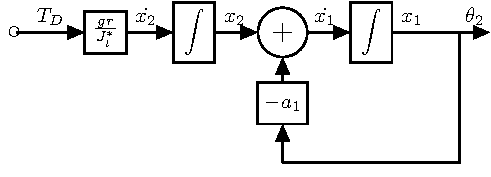
\includegraphics[scale = 1.5]{Observer4RigidBody}
\caption{State diagram for observable canonical form of rigid body model}
\label{rigidObStateDiag}
\end{figure}

Write the state equations from the state diagram:
\begin{equation}\label{rigidObservableState}
\left\{ \begin{array}{l l} 
\dot{x_1} &= x_2 - \dfrac{c_l^*}{J_l^*}x_1\\
\dot{x_2} &= \dfrac{gr}{J_l^*}T_D
\end{array}\right.\ 
\end{equation}

The output equation is 
\begin{equation}\label{rigidObservableOutput}
\theta_2 = x_1
\end{equation}

Now the observable canonical form can be constructed from equation~\ref{rigidObservableState} and equation~\ref{rigidObservableOutput}.

\begin{equation}\label{rigidObservableA}
A = \begin{bmatrix}
-\dfrac{c_l^*}{J_l^*}	&	1	\\
0	&	0
\end{bmatrix}_{2\times 2}
\end{equation}


\begin{equation}\label{rigidObservableB}
B = \begin{bmatrix}
0	\\
\dfrac{gr}{J_l^8}
\end{bmatrix}_{2\times 1}
\end{equation}


\begin{equation}\label{rigidControllableC}
C = \begin{bmatrix}
1	&	0
\end{bmatrix}_{1\times 2}
\end{equation}

\begin{equation}
D = \begin{bmatrix} 0 \end{bmatrix}
\end{equation}

% Jordan
\subsubsection{Jordan canonical form}\label{RigidJordan}
\hspace{2.5ex} To write Jordan canonical form, it is necessary to get all parameters of the system. 
From the lab manual chapter 6, we got the parameters as shown in table~\ref{rigidsystemparameters}.

\begin{table}[!htbp]
\centering
\caption{Rigid body model system parameters}
\label{rigidsystemparameters}
\begin{tabular}{|c|c|}
\hline
$J_l^*$	&	0.0331	\\	\hline
$c_l^*$	&	0.059\\	\hline
$gr$	&	1.5	\\ \hline
\end{tabular}
\end{table}

Rewrite equation~\ref{laplacerigidbody2}:
\begin{equation}\label{rigidJordanTF}
\theta_2(s) =\dfrac{gr}{J_l^* s^2 + c_l^* s} \cdot T_D(s) = \dfrac{1.5}{0.0331s^2+0.059s} T_D(s) = \dfrac{45.32}{s^2+1.782s} T_D(s)
\end{equation}

Use partial fraction technique, 
\begin{equation}\label{rigidJordanPartial}
\dfrac{\theta_2(s)}{T_D(s)} = \dfrac{25.43}{s} + \dfrac{-25.43}{s+1.782}
\end{equation}

Now Jordan canonical form can be constructed. 

\begin{equation}\label{rigidJordanA}
A = \begin{bmatrix}
0	&	0	&	\\
0	&	-1.782	
\end{bmatrix}_{2\times 2}
\end{equation}

\begin{equation}\label{rigidJordanB}
B = \begin{bmatrix}
1	\\
1
\end{bmatrix}_{2\times 1}
\end{equation}

\begin{equation}\label{rigidJordanC}
C = \begin{bmatrix}
25.43	&	-25.43
\end{bmatrix}_{1\times 2}
\end{equation}


\begin{equation}
D = \begin{bmatrix} 0 \end{bmatrix}
\end{equation}



% Flexible drive model
\subsection{Flexible drive model}
% Controllable
\subsubsection{Controllable canonical form}
\hspace{2.5ex}Start with transfer function. 
\begin{equation}\label{FlexibleControllable}
\dfrac{\theta_2(s)}{T_D(s)} = \dfrac{1}{D(s)} \cdot kgr^{-1}=\dfrac{k/(gr\cdot J_d^*\cdot J_l)}{D_3(s)}
\end{equation}
where 
\begin{equation}
D_3(s) = s^4 + \dfrac{J_d^*c_2 + J_lc_1}{J_d^*J_l} s^3 + \dfrac{J_d^*k + J_l gr^{-2}k c_1c_2}{J_d^*J_l}s^2 +\dfrac{(c_1k + c_2 gr^{-2})k}{J_d^*J_l}s
\end{equation}

From equation~\ref{FlexibleControllable}, the system can be converted into the structure shown in figure~\ref{FlexibleControllableChart}. In other words, $\dfrac{Z(s)}{T_D(s)} = \dfrac{1}{D_3(s)} \longrightarrow D_3(s) Z(s) = T_D$. 
\begin{figure}[!htbp]
\centering
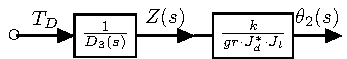
\includegraphics[scale = 1.5]{ControllableStateDiagram}
\caption{State diagram for controllable canonical form of flexible drive model}
\label{FlexibleControllableChart}
\end{figure}

So, it can be written that 
\begin{equation} \label{ControllableZ}
Z^{(4)} + \left(\dfrac{J_d^*c_2 + J_l c_1}{J_d^*J_l}\right)Z^{(3)} + \left(\dfrac{J_d^* k + J_l gr^{-2} k + c_1 c_2}{J_d^* J_l}\right) Z^{''} + \dfrac{(c_1 k +c_2 gr^{-2})k}{J_d^* J_l} Z^{'} = T_D
\end{equation}

From equation~\ref{ControllableZ}, it is clear that $a_3 = \dfrac{J_d^*c_2 + J_l c_1}{J_d^*J_l}$, $a_2 = \dfrac{J_d^* k + J_l gr^{-2} k + c_1 c_2}{J_d^* J_l}$, $a_1 = \dfrac{(c_1 k +c_2 gr^{-2})k}{J_d^* J_l} $, and $a_0 = 0$.

Let $\left\{ \begin{array}{l l}
x_1 &= Z	\\
x_2 &= \dot{Z}	\\
x_3	&= \ddot{Z}	\\
x_4 &= Z^{(3)}	\\
\end{array}\right.\ 
\Longrightarrow
\left\{ \begin{array}{l l}
\dot{x_1} &= x_2	\\
\dot{x_2} &= x_3	\\
\dot{x_3}	&= x_4	\\
\dot{x_4} &= Z^{(4)}	\\
\end{array}\right.\ 
 \therefore Z^{(4)} = T_D - a_3 x_4 - a_2 x_3 - a_1 x_2$
 
The state equations for controllable canonical form are
\begin{equation}\label{flexibleControllableState}
\left\{ \begin{array}{l l} 
\dot{x_1} &= x_2\\
\dot{x_2} &= x_3 \\
\dot{x_3} &= x_4\\
\dot{x_4} &= T_D - a_3 x_4 - a_2 x_3 - a_1 x_2
\end{array}\right.\ 
\end{equation}

In addition, from figure~\ref{FlexibleControllableChart}, $\dfrac{\theta_2(s)}{Z(s)} = \dfrac{k}{gr J_d^* J_l}$; therefore, $\theta_2(s) = \dfrac{k}{gr J_d^* J_l} Z(s)$. So the output equation is 
\begin{equation}\label{flexibleControllableOutput}
\theta_2 = \dfrac{k}{gr J_d^* J_l} x_1
\end{equation}

Now controllable canonical form can be constructed from equation~\ref{flexibleControllableState} and equation~\ref{flexibleControllableOutput}. 

\begin{equation}\label{flexibleControllableA}
A = \begin{bmatrix}
0	&	1	&	0	&	0	\\
0	&	0	&	1	&	0	\\
0	&	0	&	0	&	1	\\
0	&	-a_1	&	-a_2	&	-a_3
\end{bmatrix}_{4\times 4}
\end{equation}
where $a_1 = \dfrac{(c_1 k +c_2 gr^{-2})k}{J_d^* J_l} $, $a_2 = \dfrac{J_d^* k + J_l gr^{-2} k + c_1 c_2}{J_d^* J_l}$, and $a_3 = \dfrac{J_d^*c_2 + J_l c_1}{J_d^*J_l}$.

\begin{equation}\label{flexibleControllableB}
B = \begin{bmatrix}
0	\\
0	\\
0	\\
1
\end{bmatrix}_{4\times 1}
\end{equation}

\begin{equation}\label{flexibleControllableC}
C = \begin{bmatrix}
\frac{k}{grJ_d^*J_l}	&	0	&	0	&	0
\end{bmatrix}_{1\times 4}
\end{equation}

\begin{equation}
D = \begin{bmatrix} 0 \end{bmatrix}
\end{equation}

% Observable
\subsubsection{Observable canonical form}
\hspace{2.5ex}
From figure~\ref{FlexibleControllableChart}, the open-loop transfer function can be written as $D_3(s) \theta_2(s) = \dfrac{k}{gr\cdot J_d^* \cdot J_l} T_D(s)$. In other words, 
\begin{equation}
s^4Q\theta_2(s) + s^3 a_3 \theta_2(s) + s^2 a_2 \theta_2(s) + s a_1 \theta_2(s) = \dfrac{k}{gr\cdot J_d^* \cdot J_l}T_D(s)
\end{equation}
where $a_1 = \dfrac{(c_1 k +c_2 gr^{-2})k}{J_d^* J_l} $, $a_2 = \dfrac{J_d^* k + J_l gr^{-2} k + c_1 c_2}{J_d^* J_l}$, and $a_3 = \dfrac{J_d^*c_2 + J_l c_1}{J_d^*J_l}$.

Let $b_0 = \dfrac{k}{gr\cdot J_d^* \cdot J_l}$, so 
\begin{equation}\label{flexibleObservableTF}
\theta_2(s) = \dfrac{1}{s^4}(b_0 T_D(s)) - \dfrac{1}{s^3} a_1\theta_2(s) - \dfrac{1}{s^2}(a_2 \theta_2(s)) - \dfrac{1}{s}(a_3 \theta_2(s))
\end{equation}

From equation~\ref{flexibleObservableTF}, the state diagram can be found as figure~\ref{ObStateDiag}.

\begin{figure}[!htbp]
\centering
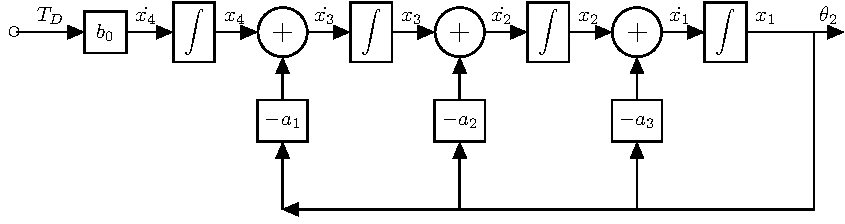
\includegraphics{ObserverStateDiagram}
\caption{Observable canonical form state diagram}
\label{ObStateDiag}
\end{figure}

Write the state equations from the state diagram:
\begin{equation}\label{flexibleObservableState}
\left\{ \begin{array}{l l} 
\dot{x_1} &= x_2 - a_3 x_1\\
\dot{x_2} &= x_3 - a_2 x_1\\
\dot{x_3} &= x_4 - a_1 x_1\\
\dot{x_4} &= b_0 T_D
\end{array}\right.\ 
\end{equation}

The output equation is 
\begin{equation}\label{flexibleObservableOutput}
\theta_2 = x_1
\end{equation}

Now observable canonical form can be constructed from equation~\ref{flexibleObservableState} and equation~\ref{flexibleObservableOutput}. 


\begin{equation}\label{flexibleObservableA}
A = \begin{bmatrix}
-a_3	&	1	&	0	&	0	\\
-a_2	&	0	&	1	&	0	\\
-a_1	&	0	&	0	&	1	\\
0	&	0	&	0	&	0
\end{bmatrix}_{4\times 4}
\end{equation}
where where, $a_1 = \dfrac{(c_1 k +c_2 gr^{-2})k}{J_d^* J_l} $, $a_2 = \dfrac{J_d^* k + J_l gr^{-2} k + c_1 c_2}{J_d^* J_l}$, and $a_3 = \dfrac{J_d^*c_2 + J_l c_1}{J_d^*J_l}$.


\begin{equation}\label{flexibleObservableB}
B = \begin{bmatrix}
0	\\
0	\\
0	\\
b_0
\end{bmatrix}_{4\times 1}
\end{equation}
where $b_0 = \dfrac{k}{gr\cdot J_d^* \cdot J_l}$.


\begin{equation}\label{flexibleControllableC}
C = \begin{bmatrix}
1	&	0	&	0	&	0
\end{bmatrix}_{1\times 4}
\end{equation}

\begin{equation}
D = \begin{bmatrix} 0 \end{bmatrix}
\end{equation}

%Jordan 
\subsubsection{Jordan canonical form}
\hspace{2.5ex}To write Jordan canonical form, it needs to find poles of characteristic polynomial. It is much more easy to find using Matlab. Besides, to write Jordan canonical form, it is necessary to get all parameters of the system. 

From the system identification practice, we got the parameters as shown in table~\ref{systemparameters}. 

\begin{table}[!htbp]
\centering
\caption{Flexible drive model system parameters}
\label{systemparameters}
\begin{tabular}{|c|c|}
\hline
$J_d$	&	$4\times 10^{-4}$\\	\hline
$gr$	&	1.5	\\ \hline
$gr'$	&	1.5	\\ \hline
$Jp$	&	$5.84\times 10^{-4}$	\\ \hline
$J_d^*$	&	0.0024	\\ \hline
$k$	&	8.45 \\ \hline
$J_l$	&	0.0271	\\ \hline
$c_1$	&	0.004	\\	\hline
$c_2$	&	0.05	\\	\hline
\end{tabular}
\end{table}

Put these values into Matlab script, the Jordan canonical form can be get.
\begin{equation}\label{flexibleJordanA}
A = \begin{bmatrix}
-1.782	&	0	&	0	&	0	\\
0	&	0	&	0	&	0	\\
0	&	0	&	-0.7827-41.5089i	&	0	\\
0	&	0	&	0	&	-0.7827+41.5089i
\end{bmatrix}_{4\times 4}
\end{equation}

\begin{equation}\label{flexibleJordanB}
B = \begin{bmatrix}
1	\\
1	\\
1	\\
1
\end{bmatrix}_{4\times 1}
\end{equation}

\begin{equation}\label{flexibleJordanC}
C = \begin{bmatrix}
-25.44	&	25.44	&	0.0157	&	-0.0214
\end{bmatrix}_{1\times 4}
\end{equation}

\begin{equation}
D = \begin{bmatrix} 0 \end{bmatrix}
\end{equation}

\vspace{7ex}
%% Impulse response and step response in (1) ================Finished=============
\section{Impulse response and the step response of the system}
\subsection{Simulation}
%Rigid body
\subsubsection{Rigid body model}

% Impulse response for rigid body
\begin{figure}[!htbp]
\centering
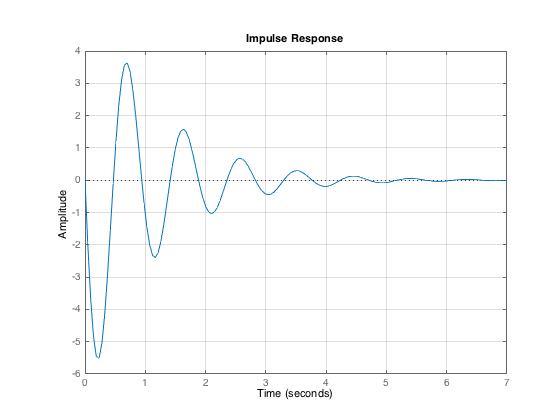
\includegraphics[scale = 0.6]{ImpulseResponseNoControl}
\caption{Close-loop impulse response of the rigid body model}
\label{ImpulseResponseNoControl}
\end{figure}

% Step response for rigid body
\begin{figure}[!htbp]
\centering
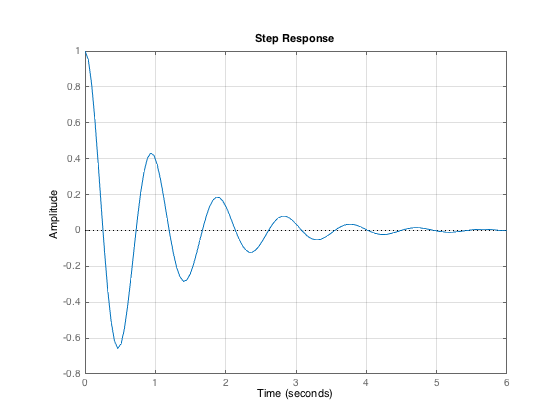
\includegraphics[scale = 0.6]{StepResponseNoControl}
\caption{Close-loop step response of the rigid body model}
\label{StepResponseNoControl}
\end{figure}

%Flexible drive
\subsubsection{Flexible drive model}

% Impulse response for flexible drive
\begin{figure}[!htbp]
\centering
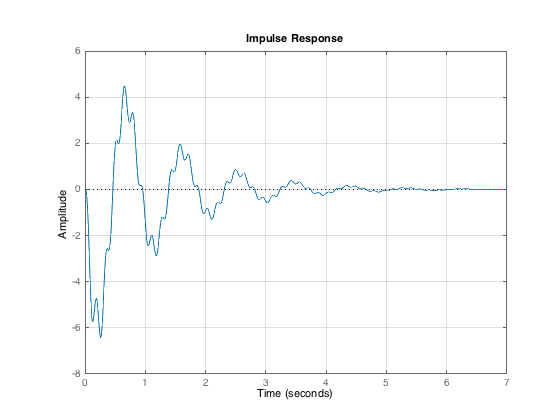
\includegraphics[scale = 0.6]{FlexibleImpulseResponseNoControl}
\caption{Close-loop impulse response of the flexible drive model}
\label{FlexibleImpulseResponseNoControl}
\end{figure}

% Step response for flexible drive
\begin{figure}[!htbp]
\centering
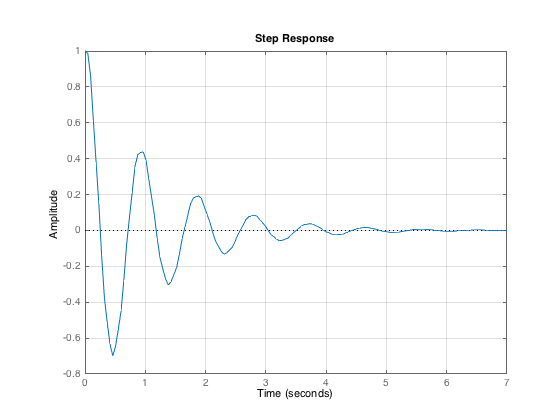
\includegraphics[scale = 0.6]{FlexibleStepResponseNoControl}
\caption{Close-loop step response of the flexible drive model}
\label{FlexibleStepResponseNoControl}
\end{figure}

\vspace{7ex}
% Lab results
\subsection{Lab results}
\begin{figure}[!htbp]
\centering
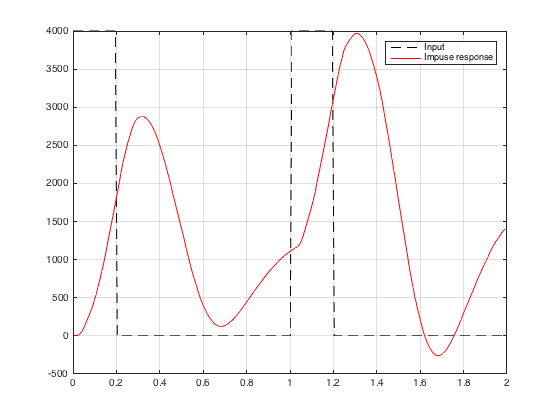
\includegraphics[scale = 0.6]{LabImpulseResponseNoControl}
\caption{Impulse response}
\label{LabImpulseResponseNoControl}
\end{figure}

\begin{figure}[!htbp]
\centering
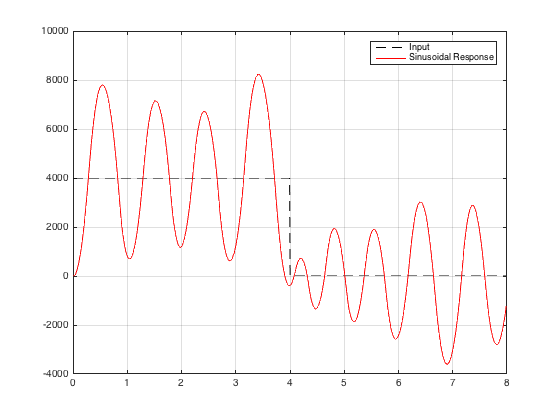
\includegraphics[scale = 0.6]{LabStepResponseNoControl}
\caption{Step response}
\label{LabStepResponseNoControl}
\end{figure}


%%Bode plot and root-locus ============================Finished =============
\section{Plot the Bode plot of the uncompensated system and root-locus of the open-loop system}
% Rigid body model 
\subsection{Rigid body model}
% bode plot
\begin{figure}[!h]
\centering
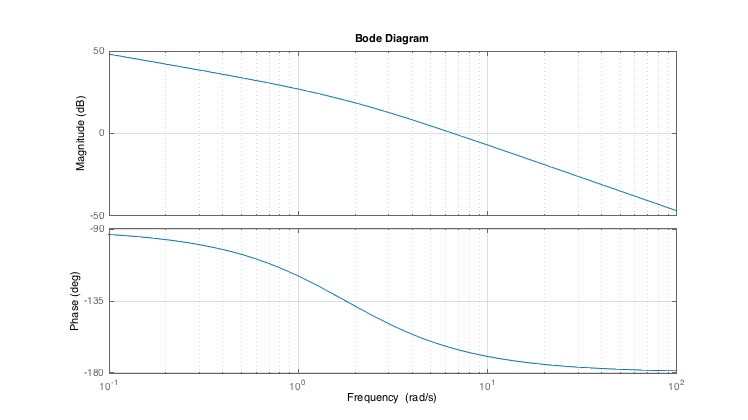
\includegraphics[width = 0.9\linewidth]{BodePlot}
\caption{Bode plot of rigid body model}
\label{BodePlot}
\end{figure}
% root locus
\begin{figure}[!h]
\centering
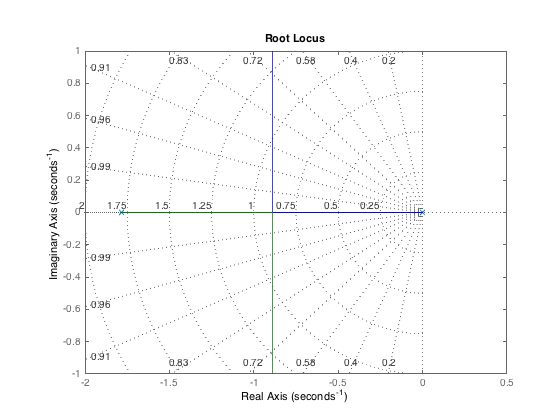
\includegraphics[width = 0.9\linewidth]{rLocus}
\caption{Root locus of rigid body model}
\label{rLocus}
\end{figure}

% Flexible drive model
\subsection{Flexible drive model}
% bode plot
\begin{figure}[!h]
\centering
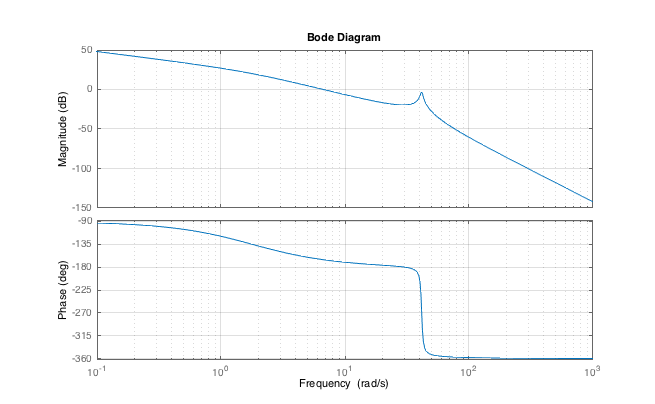
\includegraphics[width = 1\linewidth]{FlexibleBodePlot}
\caption{Bode plot of flexible drive model}
\label{FlexibleBodePlot}
\end{figure}
% root locus
\begin{figure}[!h]
\centering
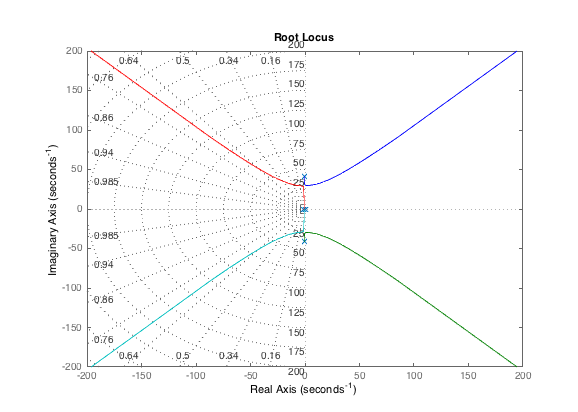
\includegraphics[width = 0.9\linewidth]{FlexiblerLocus}
\caption{Root locus of flexible drive model}
\label{FlexiblerLocus}
\end{figure}

\vspace{7ex}
%% PID or lead-lag controller================================Finished ============
\section{Design a lead-lag controller to meet certain design specification}\label{DesignRequirements}
\hspace{2.5ex} Here are the design specifications: 
\begin{enumerate}
\item[-]{$t_s \le 2s \longrightarrow \xi \omega \ge 2 $}
\item[-]{Percentage of overshoot $< 5\% \longrightarrow \xi = 0.707$}
\item[-]{$e_{ss}$ due to step input is zero $\longrightarrow$ has a $\dfrac{1}{s}$ in the forward path}
\end{enumerate}

% Rigid body model
\subsection{Rigid body model}
\hspace{2.5ex} We use sisotool in Matlab to design the lead-lag controller. To drag the root locus into the desired region, it need to add a pole at location of $-4$ and to add a zero at location of $-1.78$. Take the gain of 0.012134 to make sure the root locus is completely within the desired region. Figure~\ref{LeadLagController} is the plots of the compensated system. The lead compensator is $G_c = 0.012134\dfrac{1+0.56s}{1+0.25s}$.

\begin{figure}[!htbp]
\centering
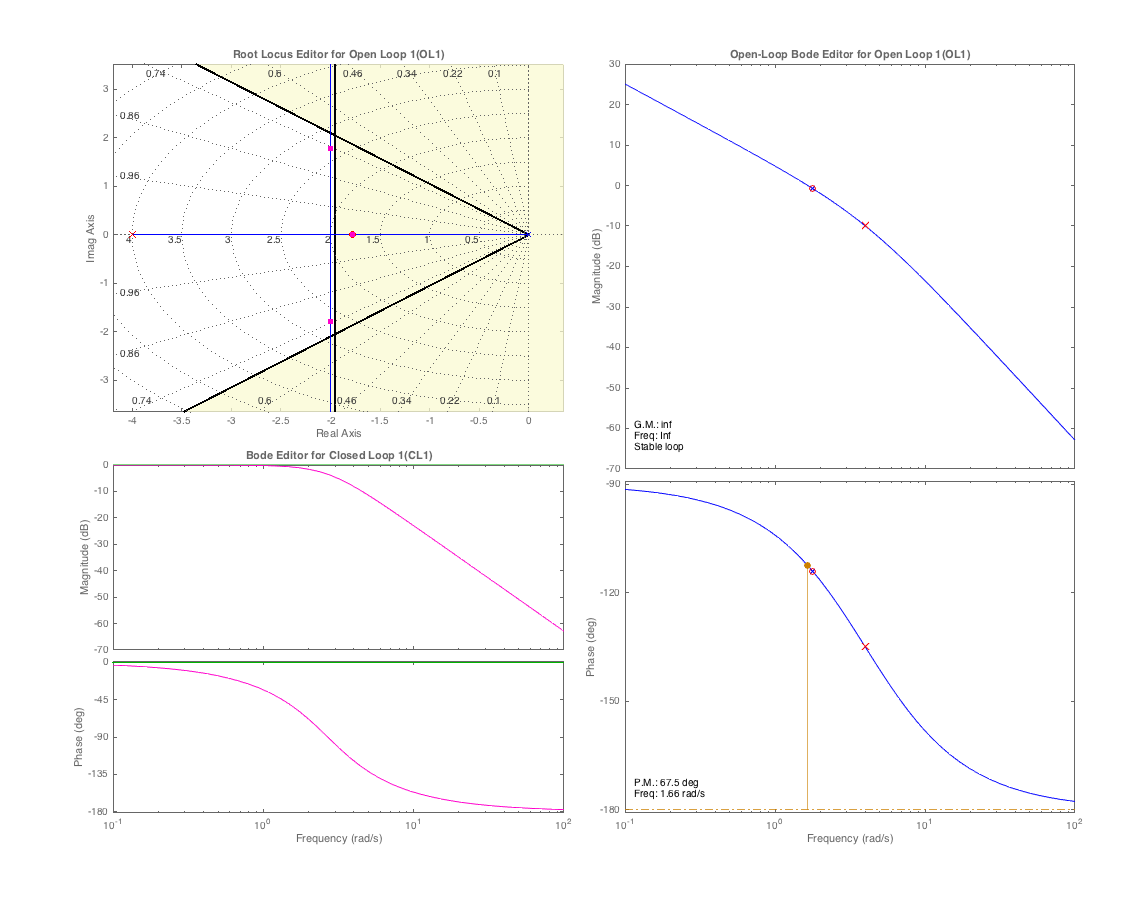
\includegraphics[width = 1\linewidth]{LeadLagController}
\caption{Lead compensator design for rigid body model}
\label{LeadLagController}
\end{figure}

% Flexible drive model
\subsection{Flexible drive model}
\hspace{2.5ex} The flexible drive model is the fourth order system. In addition to the lead controller we use in rigid body model, we need a lag controller to deal with the imaginary poles $-0.7827\pm 41.5089i$. So we put a pair of imaginary zeros to cancel out these two imaginary poles. The lead-lag compensator is $G_c = 0.012134\dfrac{(1+0.56s)[1+0.00091s+ (0.024s)^2]}{1+0.25s}$

\begin{figure}[!htbp]
\hspace{-7ex}
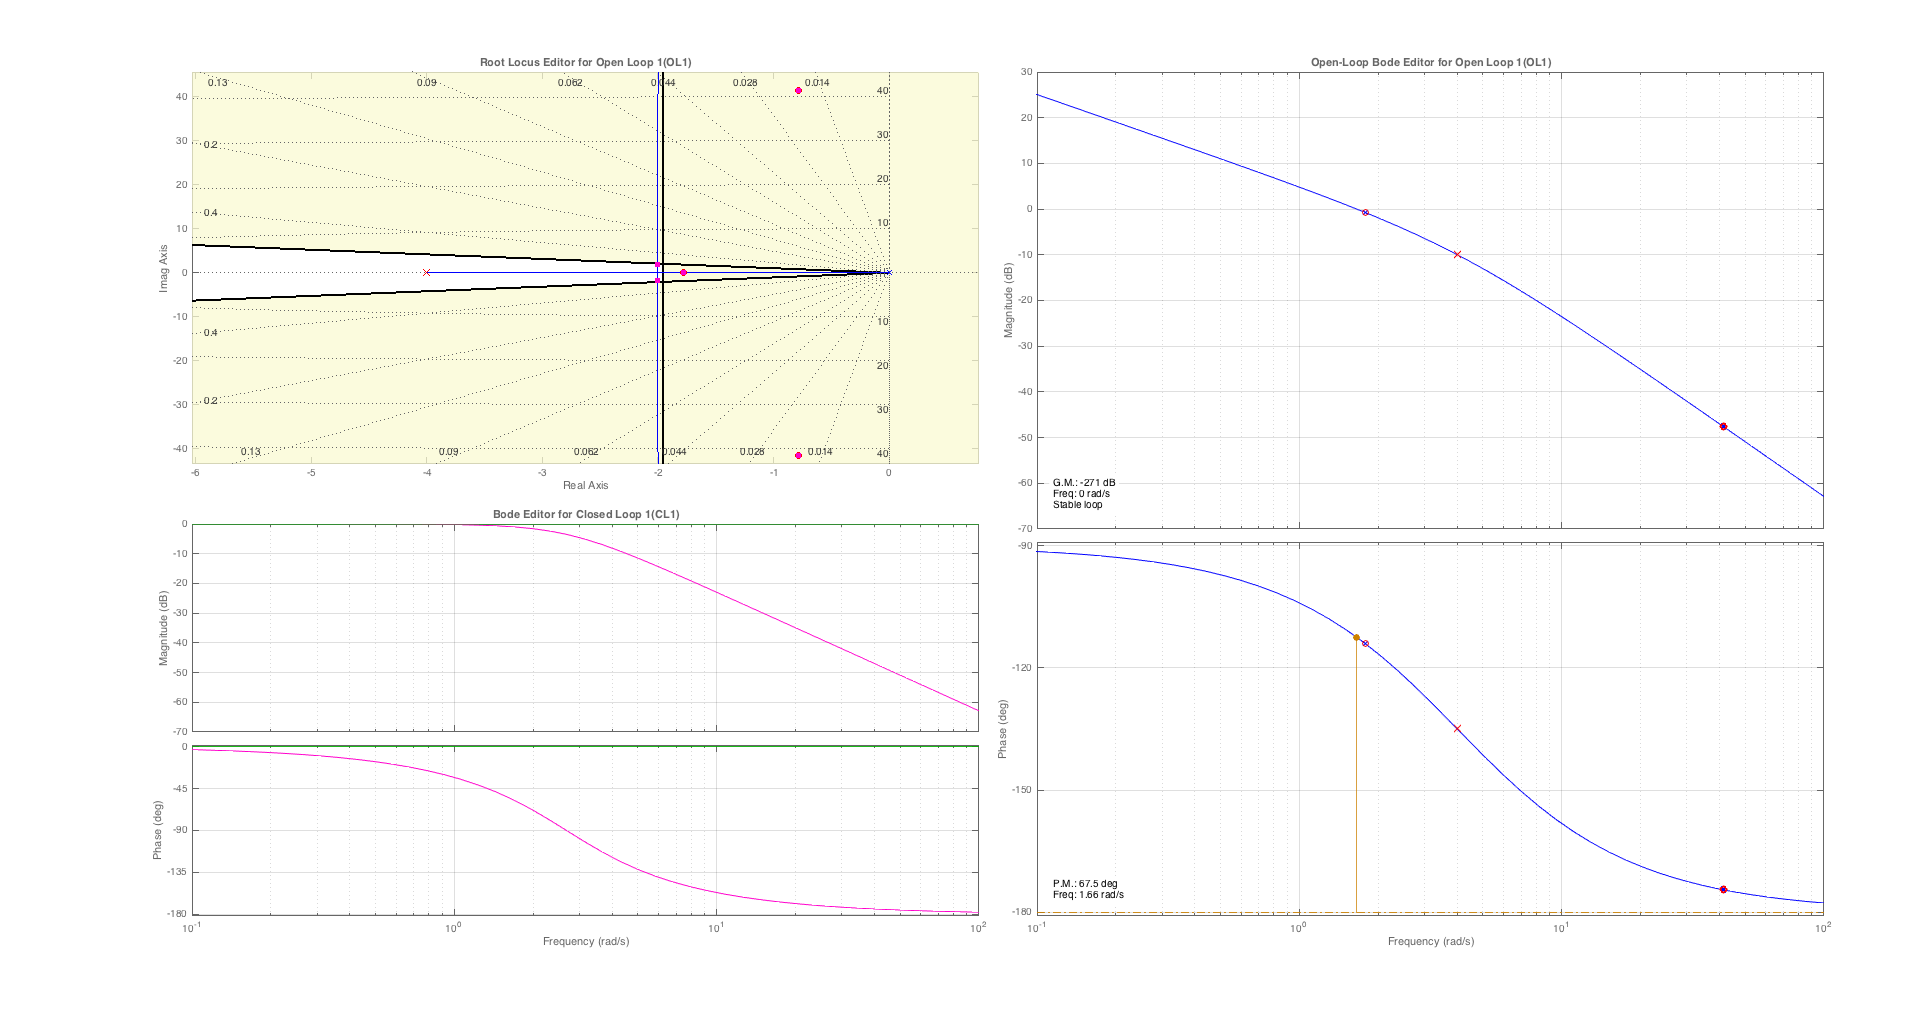
\includegraphics[width = 1.2\linewidth]{FlexibleLeadLagController}
\caption{Lead lag compensator design for flexible drive model}
\label{FlexibleLeadLagController}
\end{figure}

\vspace{7ex}
%%  Step response, square wave and sinusoidal response ==========Finished============
\section{Step, square wave, and sinusoidal response of compensated system}

% Simulation
\subsection{Simulation}
\hspace{2.5ex}
Figure~\ref{StepResponseLeadLag}, figure~\ref{CubicResponseLeadLag}, and figure~\ref{SinusoidalResponseLeadLag} are the step response, square wave response, and sinusoidal wave response respectively for the compensated system of rigid body model.

Figure~\ref{FlexibleStepResponseLeadLag}, figure~\ref{FlexibleCubicResponseLeadLag}, and figure~\ref{FlexibleSinusoidalResponseLeadLag} are the step response, square wave response, and sinusoidal wave response respectively for the compensated system of flexible drive model. 

It is clear that the responses of both model are almost identical. 

%Rigid body model
\begin{figure}[!htbp]
\centering
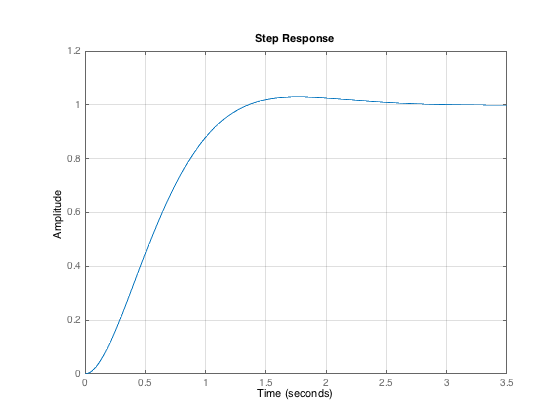
\includegraphics[scale = 0.6]{StepResponseLeadLag}
\caption{Step response of the compensated system, rigid body model}
\label{StepResponseLeadLag}
\end{figure}

\begin{figure}[!htbp]
\centering
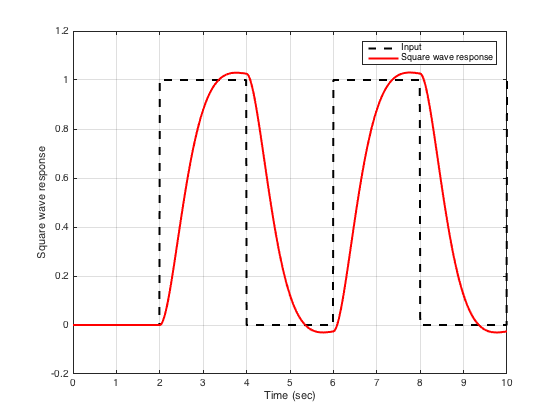
\includegraphics[scale = 0.6]{CubicResponseLeadLag}
\caption{Square wave response of the compensated system, rigid body model}
\label{CubicResponseLeadLag}
\end{figure}

\begin{figure}[!htbp]
\centering
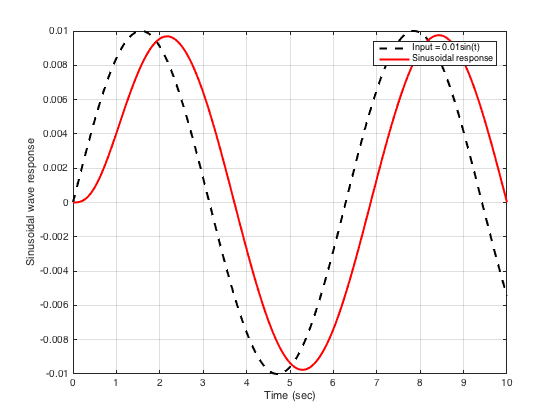
\includegraphics[scale = 0.6]{SinusoidalResponseLeadLag}
\caption{Sinusoidal response of the compensated system, rigid body model}
\label{SinusoidalResponseLeadLag}
\end{figure}

% Flexible drive model
\begin{figure}[!htbp]
\centering
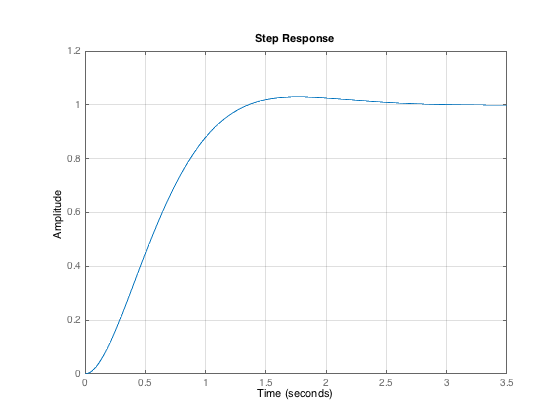
\includegraphics[scale = 0.6]{FlexibleStepResponseLeadLag}
\caption{Step response of the compensated system, flexible model}
\label{FlexibleStepResponseLeadLag}
\end{figure}

\begin{figure}[!htbp]
\centering
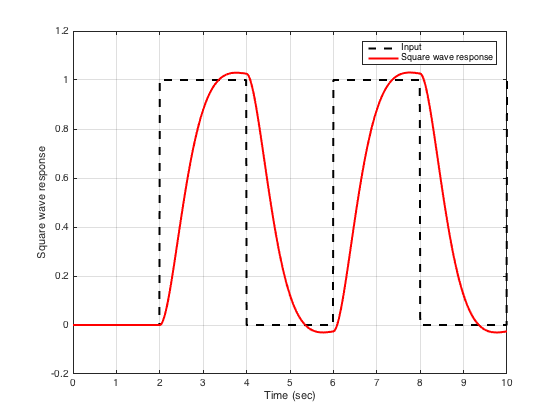
\includegraphics[scale = 0.6]{FlexibleCubicResponseLeadLag}
\caption{Square wave response of the compensated system, flexible drive model}
\label{FlexibleCubicResponseLeadLag}
\end{figure}

\begin{figure}[!htbp]
\centering
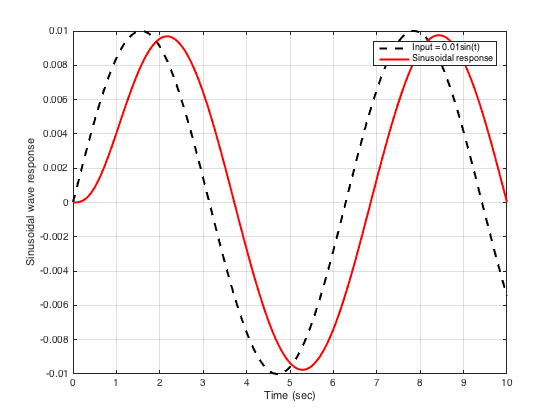
\includegraphics[scale = 0.6]{FlexibleSinusoidalResponseLeadLag}
\caption{Sinusoidal response of the compensated system, flexible drive model}
\label{FlexibleSinusoidalResponseLeadLag}
\end{figure}


% Lab result
\subsection{Lab results}
\hspace{2.5ex}We only used the compensator of rigid body model to do the lab. Therefore, figure~\ref{LabStepResponseLeadLag}, figure~\ref{LabCubicResponseLeadLag}, and figure~\ref{LabSinusoidalResponseLeadLag} shows the lab results of rigid body compensated system. 
As shown in the graph, the lab results are similar to the simulation results in response waveform. 

%Lab 
\begin{figure}[!htbp]
\centering
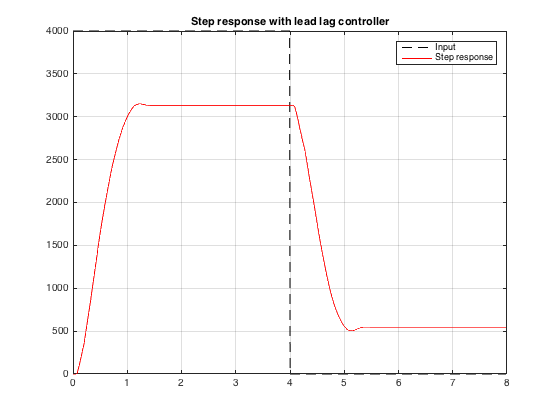
\includegraphics[scale = 0.6]{LabStepResponseLeadLag}
\caption{Step response of the compensated system, Lab result}
\label{LabStepResponseLeadLag}
\end{figure}

\begin{figure}[!htbp]
\centering
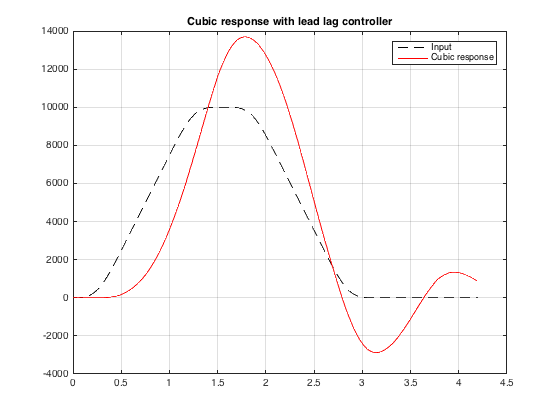
\includegraphics[scale = 0.6]{LabCubicResponseLeadLag}
\caption{Square wave response of the compensated system, Lab result}
\label{LabCubicResponseLeadLag}
\end{figure}

\begin{figure}[!htbp]
\centering
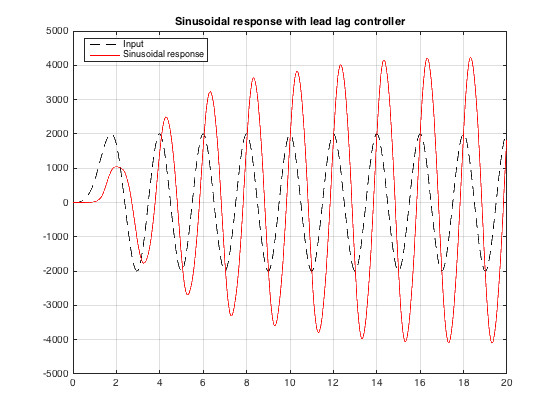
\includegraphics[scale = 0.6]{LabSinusoidalResponseLeadLag}
\caption{Sinusoidal response of the compensated system, Lab result}
\label{LabSinusoidalResponseLeadLag}
\end{figure}


%% Test robustness===========================================Finished =========
\section{Test the robustness of the compensated system}
\hspace{2.5ex}We introduced disturbance into the system to test its robustness. 
Figure~\ref{LabStepResponseLeadLagDisturbance} is the step response with lead compensator and disturbance of $2v /rad/s$.
%Lab 
%Step response
\begin{figure}[!htbp]
\centering
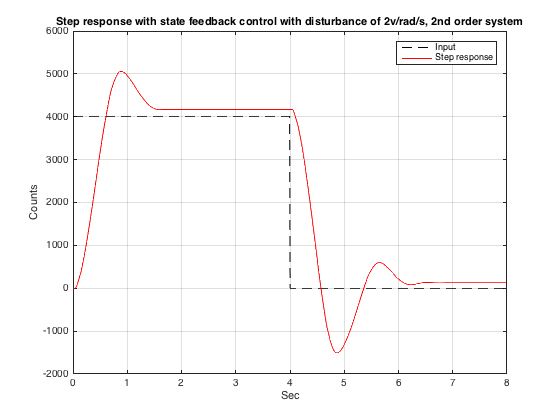
\includegraphics[scale = 0.6]{LabStepResponseLeadLagDisturbance}
\caption{Step response of the compensated system with disturbance, Lab result}
\label{LabStepResponseLeadLagDisturbance}
\end{figure}

% Cubic response
We introduced the same disturbance to the square wave response. Figure~\ref{LabCubicResponseLeadLagDisturbance}
\begin{figure}[!htbp]
\centering
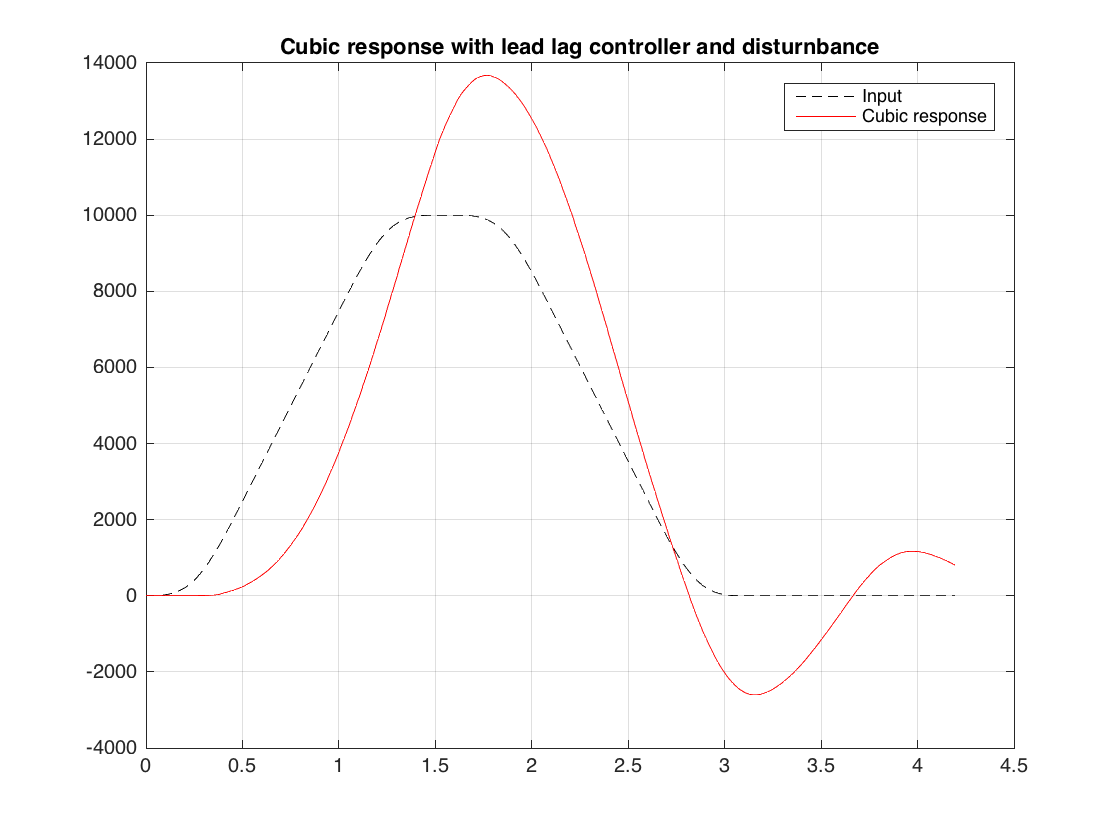
\includegraphics[scale = 0.3]{LabCubicResponseLeadLagDisturbance}
\caption{Square wave response of the compensated system with disturbance, Lab result}
\label{LabCubicResponseLeadLagDisturbance}
\end{figure}

%Sinusoidal response
For the sinusoidal response, the input sinusoidal wave had the amplitude of 2000 counts, frequency of 0.5Hz. The disturbance amplitude was $3v/rad/s$. Figure~\ref{LabSinusoidalResponseLeadLagDisturbance} is the sinusoidal response with lead compensator and disturbance. 

\begin{figure}[!htbp]
\centering
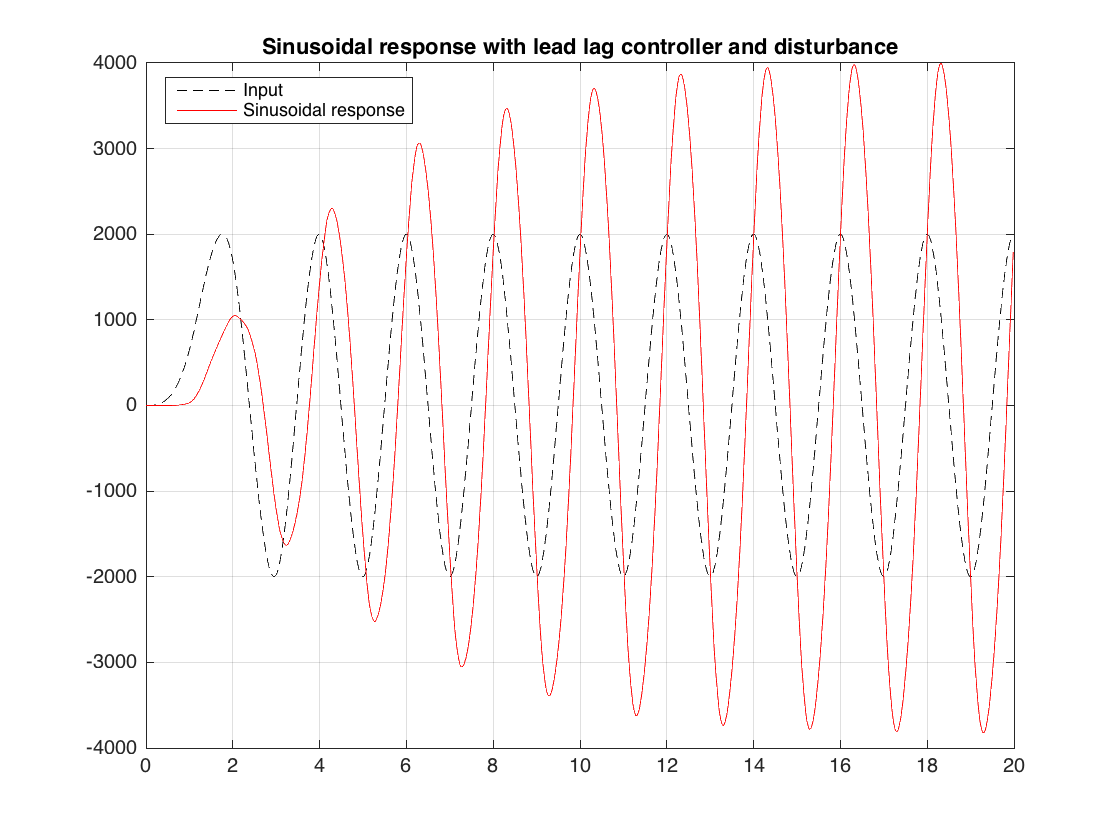
\includegraphics[scale = 0.3]{LabSinusoidalResponseLeadLagDisturbance}
\caption{Sinusoidal response of the compensated system with disturbance, Lab result}
\label{LabSinusoidalResponseLeadLagDisturbance}
\end{figure}

From the lab practice, it is clear that the compensated system was a robust system and could hold some disturbance. 



% Full state feedback control =====================================Finished ==========
\section{Design a full state feedback control to meet the design specification}
\hspace{2.5ex} As the discussion in section~\ref{DesignRequirements}, the design requirements can be translated into the values of $\xi$ and $\omega$. Here, we used the same results from section~\ref{DesignRequirements} that $\xi = 0.707$ and $\omega = 2.86$.

The characteristic equation of desired requirements is $s^2 + 2\xi \omega s + \omega^2 =0 $. Plug in the value os $\xi$ and $\omega$: 
\begin{equation}\label{characteristicEqn}
s^2 + 4.04404s + 8.1796 =0 
\end{equation}

% Rigid body model
\subsection{Rigid body model}
For rigid body model, two poles of the characteristic equation are enough to design a full state feedback controller. The equation~\ref{characteristicEqn} gives the target characteristic polynomial of $det[sI - A+BK]$, where $A$ and $B$ are discussed in section~\ref{Equations}, and $K = \begin{bmatrix} k_1 & k_2 \end{bmatrix}$. The values in $A$ and $B$ can be calculated by the parameters given in table~\ref{rigidsystemparameters}. To reiterate the equations of rigid body model: 

$A=
%A
\begin{bmatrix}
0	&	1	\\
0	&	-1.782
\end{bmatrix}
$, 
$B=
%B
\begin{bmatrix}
0\\
263.2215
\end{bmatrix} 
$, 
$C = 
\begin{bmatrix}
1 &	0
\end{bmatrix}
$,
 and $D = \begin{bmatrix} 0 \end{bmatrix}$.
 
So, 
\begin{equation}
det[sI - A+BK] = det
\begin{bmatrix}
s	&	-1	\\
263.2215k_1	&	s+1.782+263.2215k_2
\end{bmatrix} =0
\end{equation}

\begin{equation}\label{findCharacteristicEqn}
\Longrightarrow s(s+1.782+263.2215k_2) + 263.2215k_1 = 0 
\end{equation}

To make equation~\ref{findCharacteristicEqn} = equation~\ref{characteristicEqn}, get $k_1 = 0.0311$ and $k_2 = 0.0086$. 
\begin{equation}\label{K4rigid}
\mathbf{K} = 
\begin{bmatrix}
0.0311	&	0.0086
\end{bmatrix}
\end{equation}

% Flexible drive model
\subsection{Flexible drive model}
\hspace{2.5ex}
The flexible drive model is a fourth order system; therefore, four poles are needed to define the controller. In addition to the requirements described in equation~\ref{characteristicEqn}, we set two more poles far away from the imaginary axis in s-plain, say $-15$ and $-20$. These two additional poles are not dominant; therefore, they decay quickly and will not affect the system too much. 

The calculation of fourth order system is very complicated. We used the same method to find $\mathbf{K}$ for flexible drive model as we did for rigid body model but worked in a m-file so that Matlab does the calculation.

The output of Matlab is as followed.

\begin{verbatim}
>> K

K =

   -0.6145    0.0163    0.9272   -0.0225
\end{verbatim}

\begin{equation}\label{K4flexible}
\mathbf{K} = 
\begin{bmatrix}
-0.6145	&	0.0163	&	0.9272	&	-0.0225
\end{bmatrix}
\end{equation}


%Obtain the step, square wave and sinusoidal responses with arbitrary initial conditions and compare the results with those in (7).=====================================Finished==========
\section{Obtain the responses for full state feedback controlled system}
\subsection{Simulation}
% Rigid body model
% Step response
\begin{figure}[!htbp]
\centering
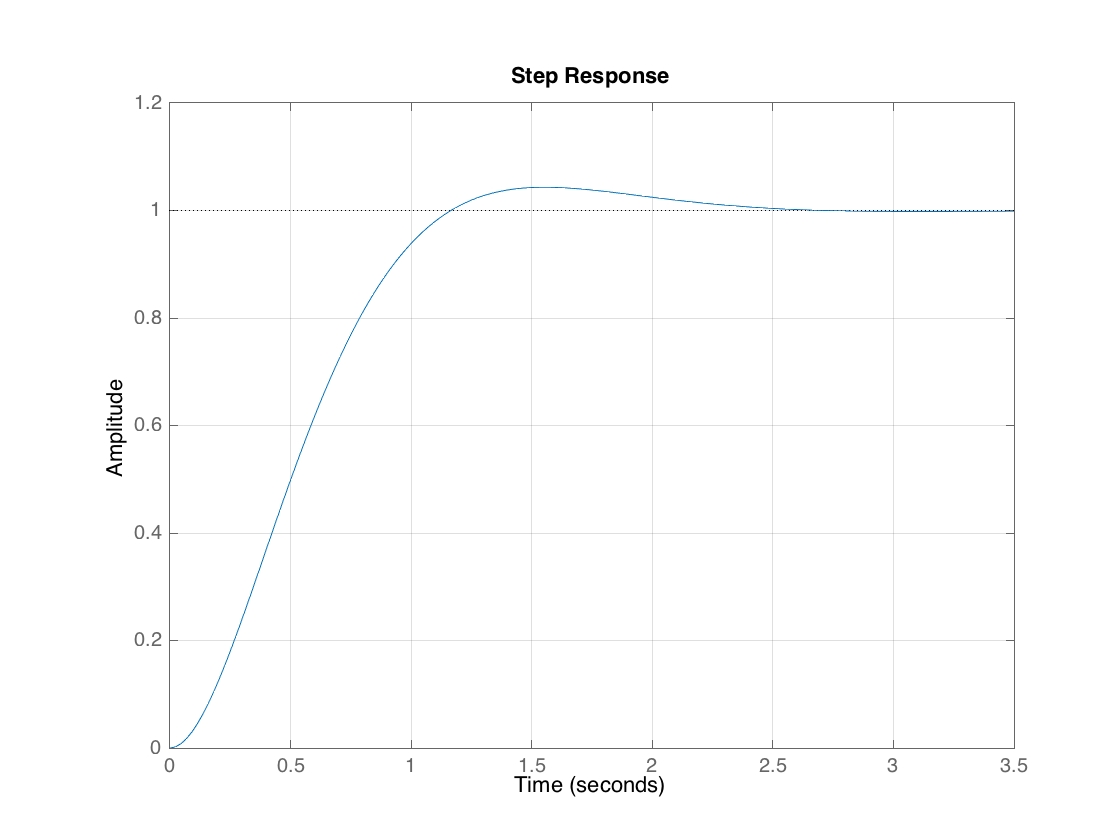
\includegraphics[scale = 0.3]{StepResponseStateFeedback}
\caption{Step response of the state feedback controlled system, rigid body model}
\label{StepResponseStateFeedback}
\end{figure}

%Cubic
\begin{figure}[!htbp]
\centering
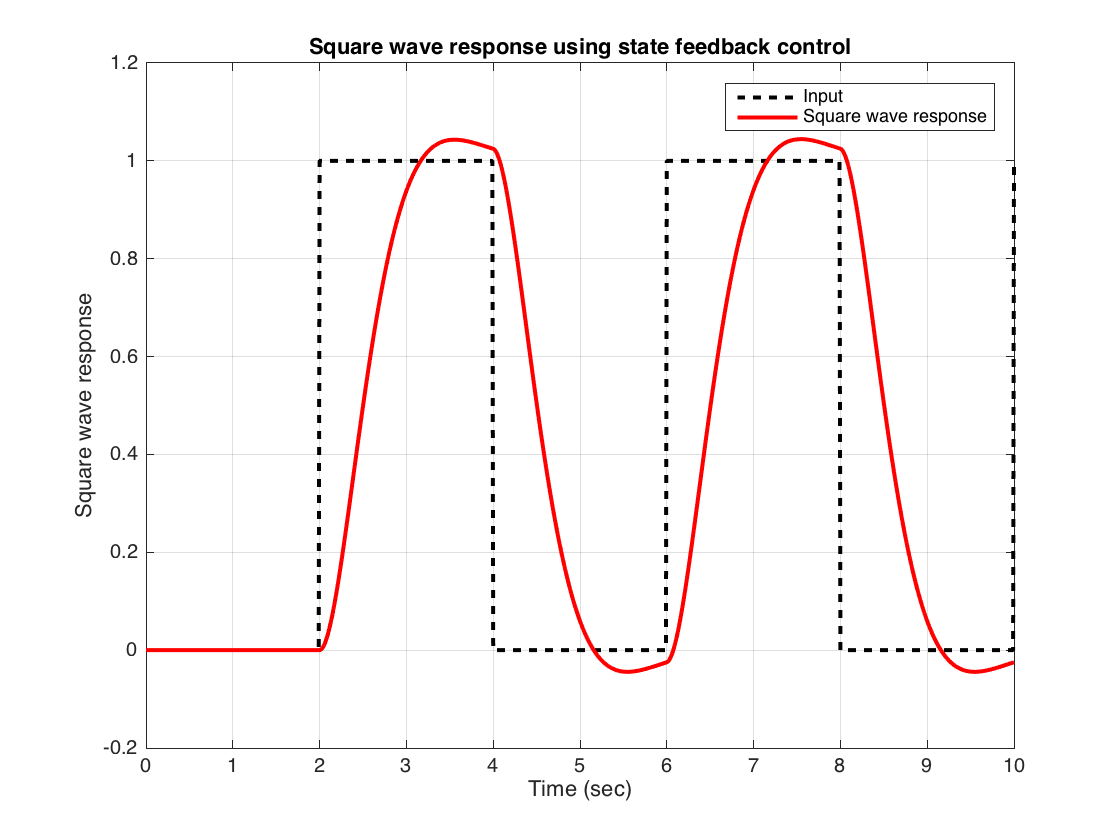
\includegraphics[scale = 0.3]{CubicResponseStateFeedback}
\caption{Square wave response of the state feedback controlled system, rigid body model}
\label{CubicResponseStateFeedback}
\end{figure}

%Sinusoidal
\begin{figure}[!htbp]
\centering
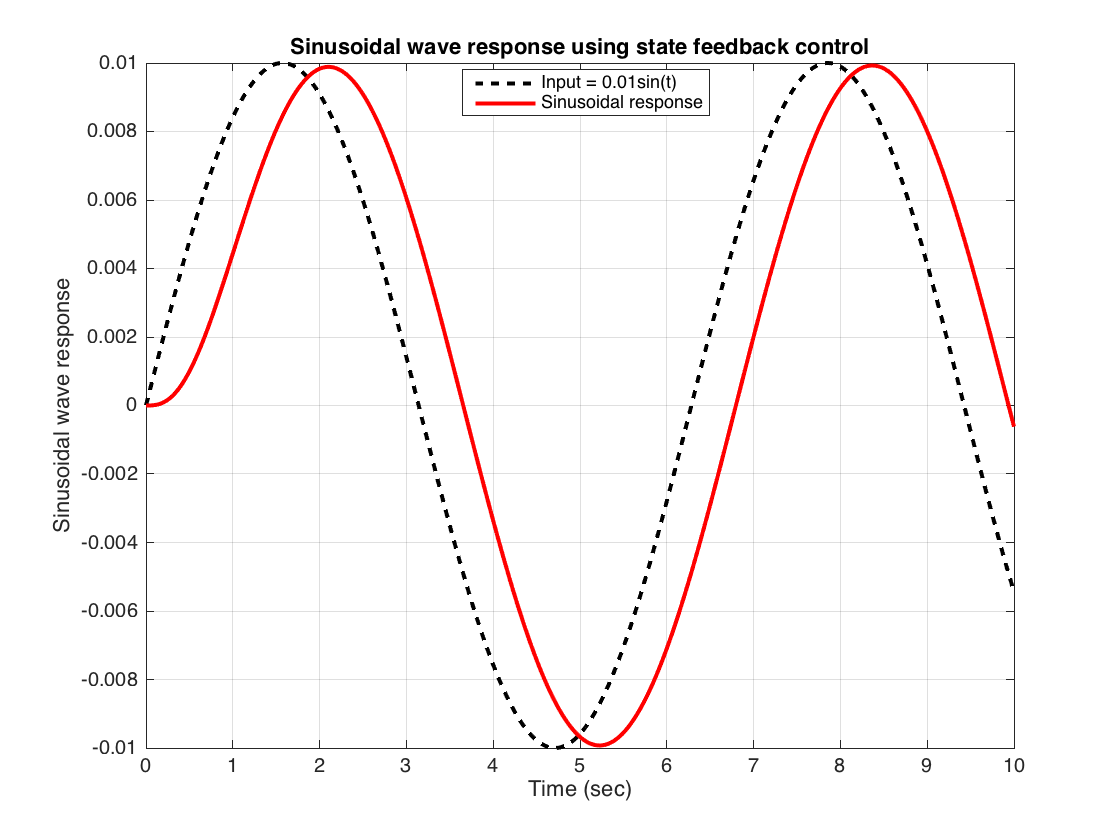
\includegraphics[scale = 0.3]{SinusoidalResponseStateFeedback}
\caption{Sinusoidal wave response of the state feedback controlled system, rigid body model}
\label{SinusoidalResponseStateFeedback}
\end{figure}


% Flexible drive model
% Step response
\begin{figure}[!htbp]
\centering
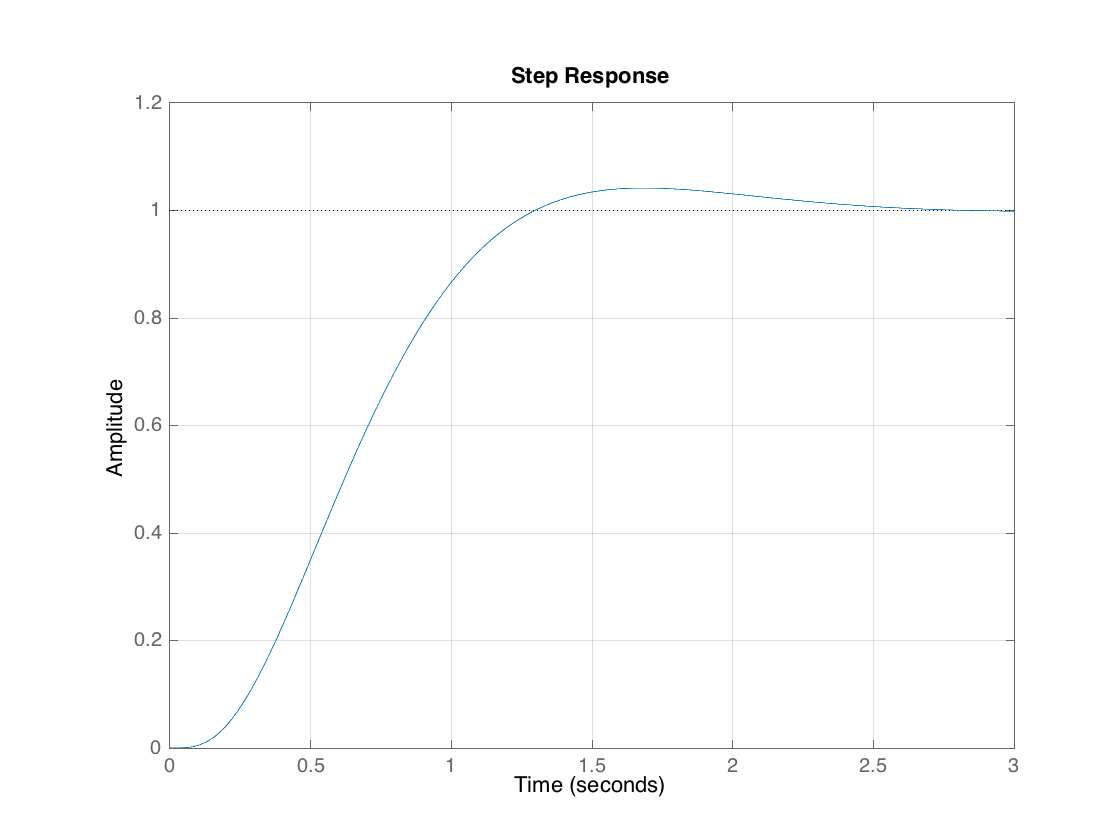
\includegraphics[scale = 0.3]{FlexibleStepResponseStateFeedback}
\caption{Step response of the state feedback controlled system, flexible drive model}
\label{FlexibleStepResponseStateFeedback}
\end{figure}

%Cubic
\begin{figure}[!htbp]
\centering
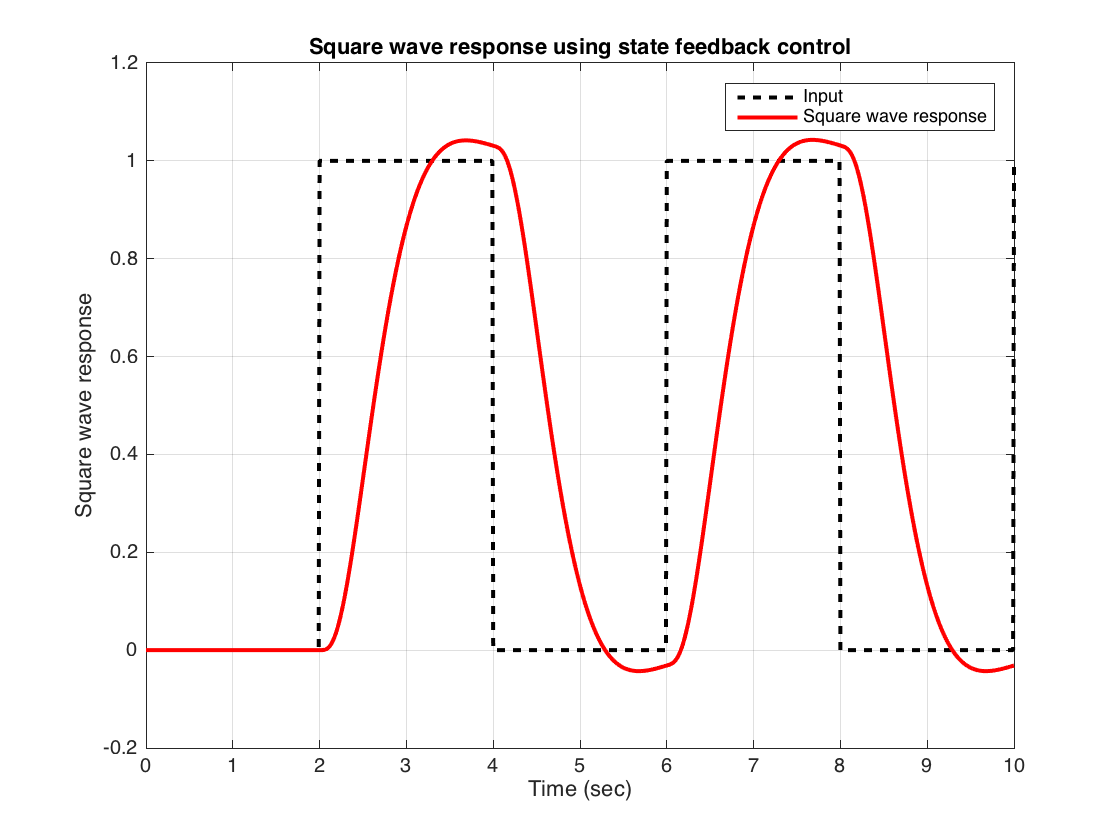
\includegraphics[scale = 0.3]{FlexibleCubicResponseStateFeedback}
\caption{Square wave response of the state feedback controlled system, flexible drive model}
\label{CubicResponseStateFeedback}
\end{figure}

%Sinusoidal
\begin{figure}[!htbp]
\centering
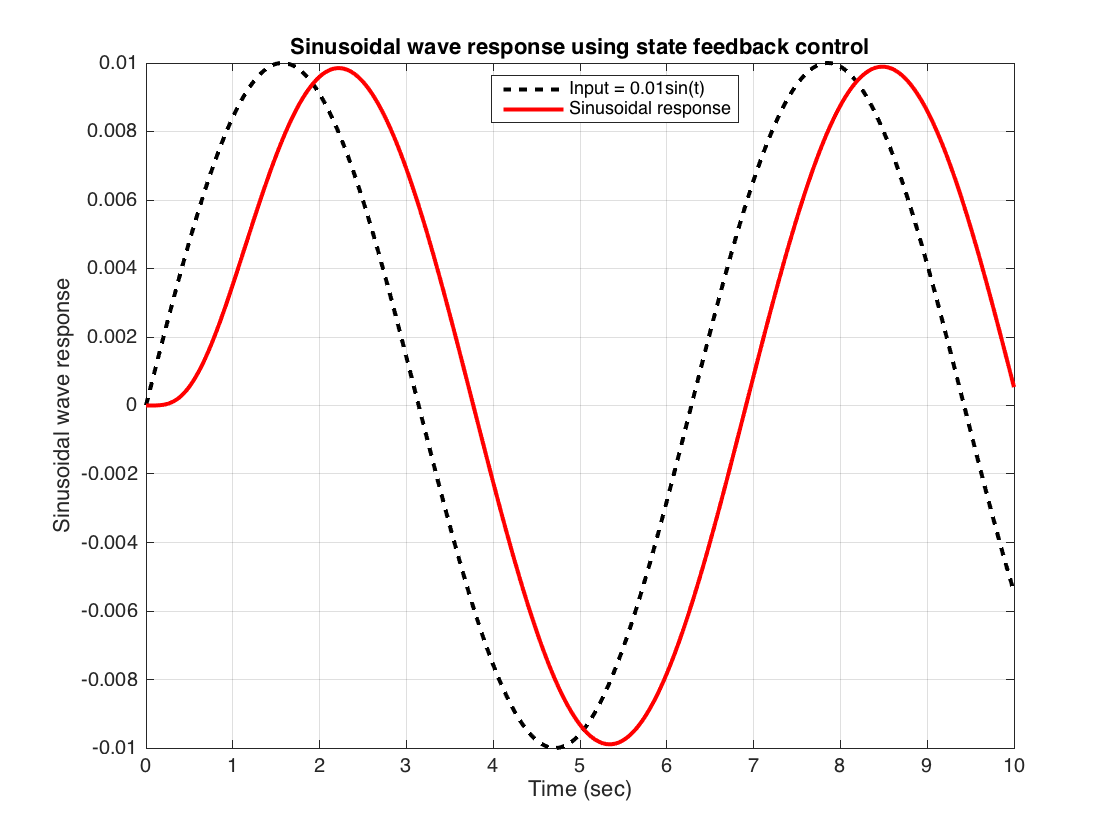
\includegraphics[scale = 0.3]{FlexibleSinusoidalResponseStateFeedback}
\caption{Sinusoidal wave response of the state feedback controlled system, flexible drive model}
\label{FlexibleSinusoidalResponseStateFeedback}
\end{figure}


% Lab results
\subsection{Lab results}
\hspace{2.5ex} Figure~\ref{LabStepResponseStateFeedback} is the step response of the controlled system. The controller was set according to rigid body model. From the result, the steady state error was much larger than our expectation. We tried to adjust $K_{pf}$, and the result in figure~\ref{LabStepResponseStateFeedback} was the best result we could get. It did meet other two design requirements which are $t_s \le 2s$ and $P.O. < 5s$, but the requirement of zero steady state error was not satisfied. The same situation happened in fourth order controller as shown in figure~\ref{LabStepResponseStateFeedback4thOrder}. One possible reason could be the system we simulated was not the same as we did for the lab. Because two teams worked in the same station, the system could be changed a little bit by the other team. Therefore, the system was not the expected one we did for our simulation. 

Except for the zero $e_{ss}$ problem, the state feedback controller worked well. 

% Step response
\begin{figure}[!htbp]
\centering
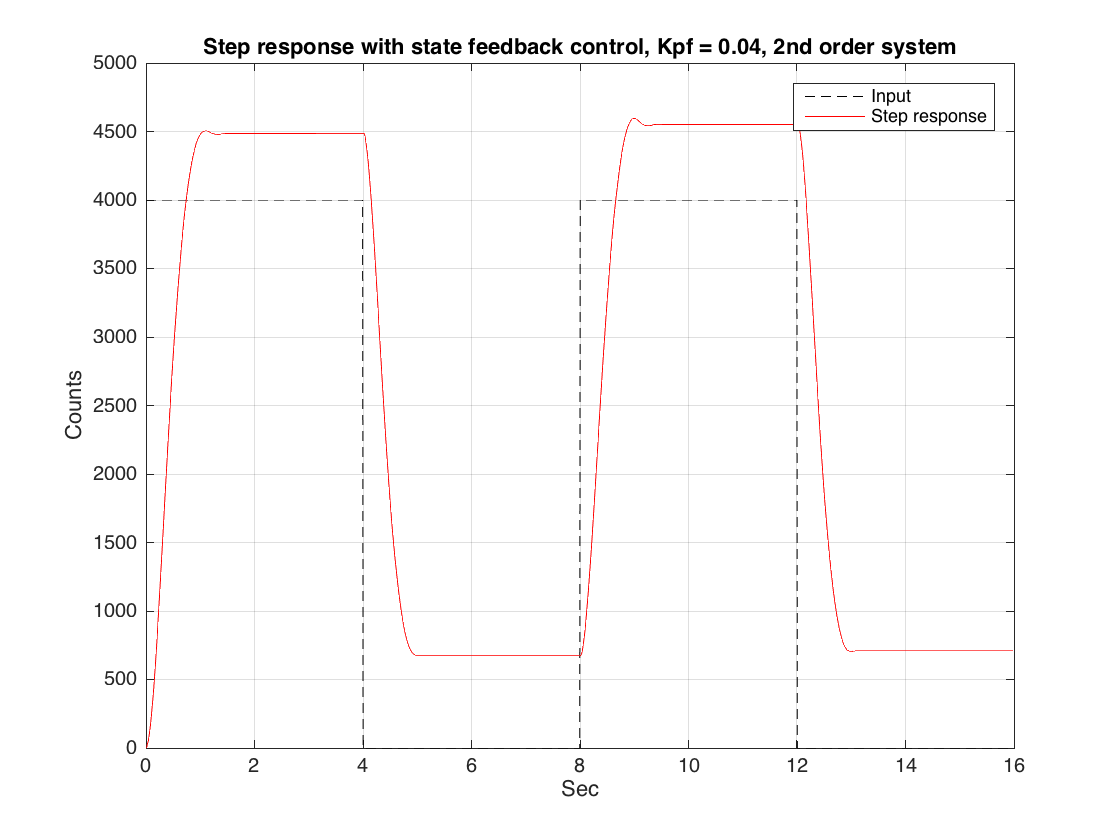
\includegraphics[scale = 0.3]{LabStepResponseStateFeedback}
\caption{Step response of the state feedback controlled system, Lab result of second order system}
\label{LabStepResponseStateFeedback}
\end{figure}

\begin{figure}[!htbp]
\centering
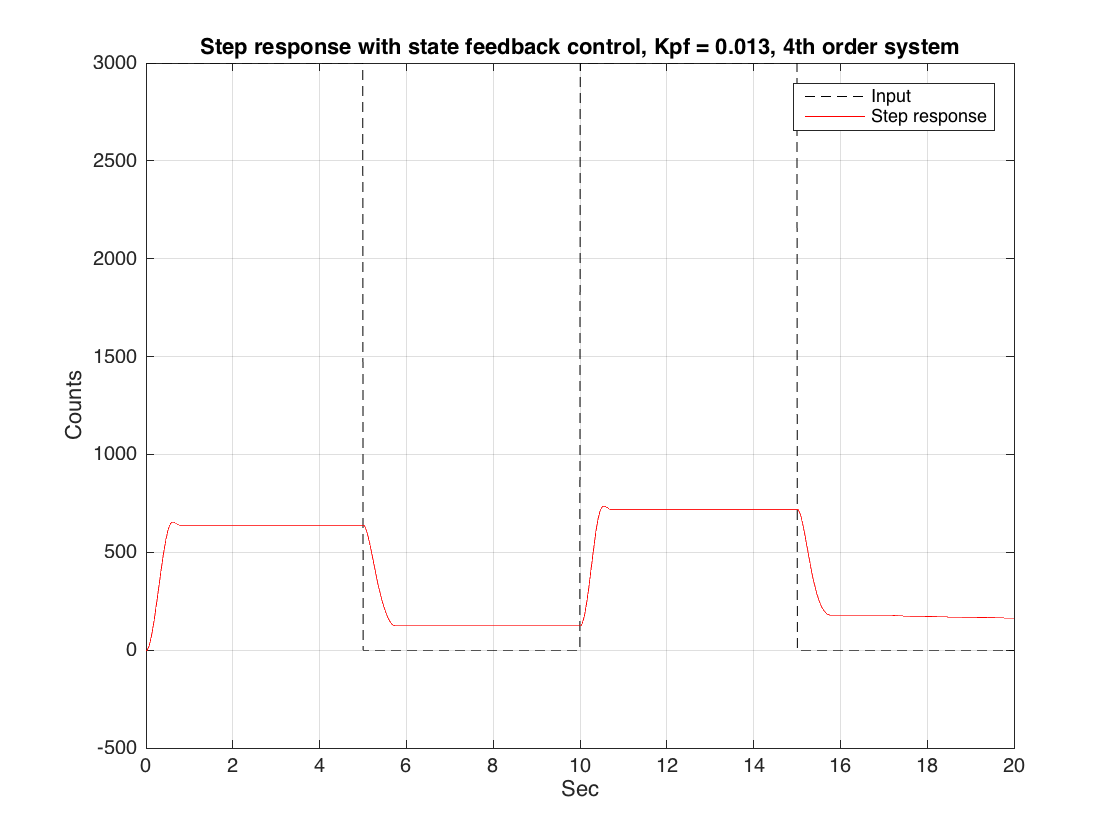
\includegraphics[scale = 0.3]{LabStepResponseStateFeedback4thOrder}
\caption{Step response of the state feedback controlled system, Lab result of fourth order system}
\label{LabStepResponseStateFeedback4thOrder}
\end{figure}


%Cubic response
\begin{figure}[!htbp]
\centering
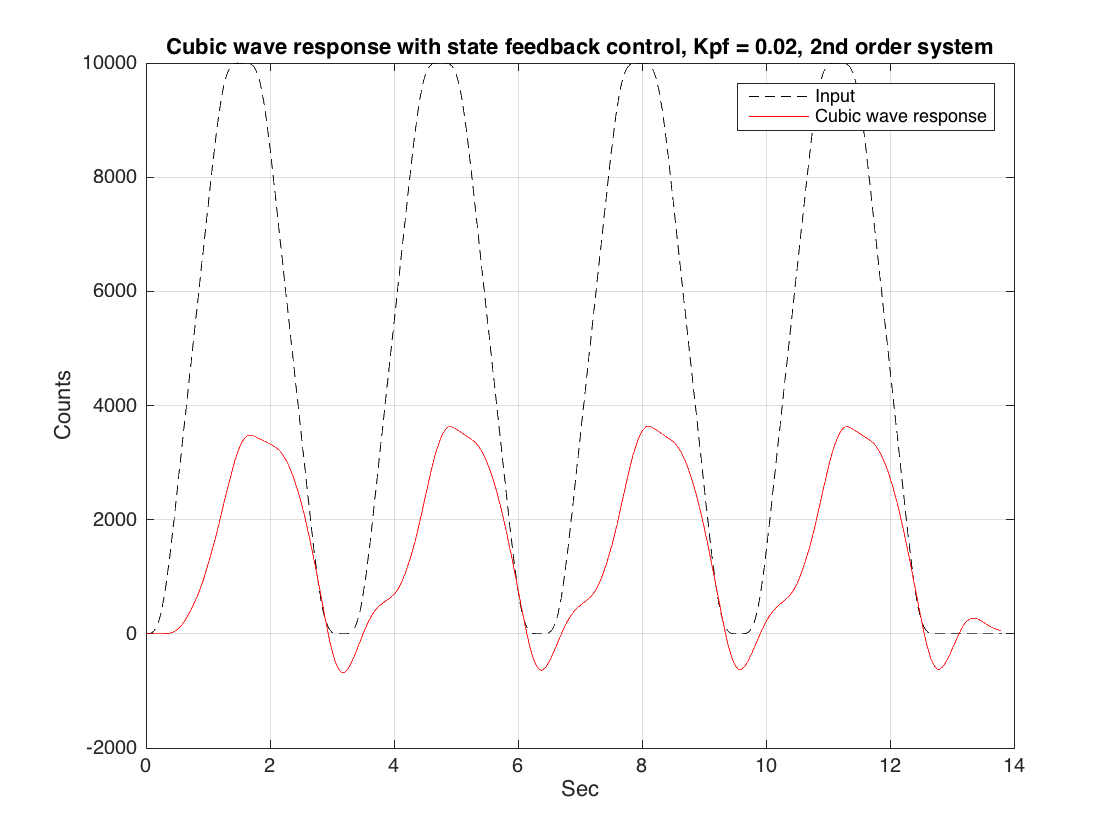
\includegraphics[scale = 0.3]{LabCubicResponseStateFeedback}
\caption{Square wave response of the state feedback controlled system, Lab result of second order system}
\label{LabCubicResponseStateFeedback}
\end{figure}

% Sinusoidal response
\begin{figure}[!htbp]
\centering
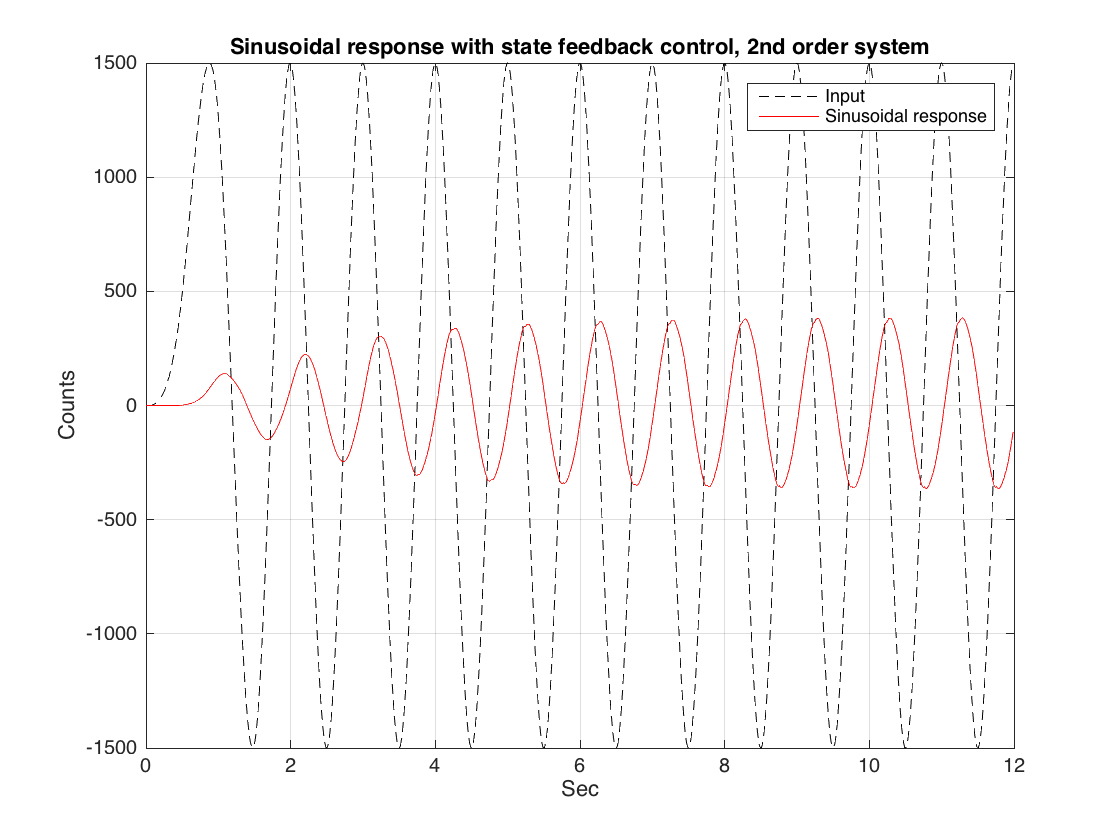
\includegraphics[scale = 0.3]{LabSinusoidalResponseStateFeedback}
\caption{Sinusoidal wave response of the state feedback controlled system, Lab result of second order system}
\label{LabSinusoidalResponseStateFeedback}
\end{figure}


\newpage
%% Design a full-order and a reduced-order observer and obtain step and sinusoidal responses
% ====================================================Finished=========
\section{Design a full-order and a reduced-order observer}
% Full order observer
\subsection{Full-order observer}
% Rigid body model
\subsubsection{Rigid body model}
\hspace{2.5ex}
In full state feedback controller design, we put the desired pole at $-2.022\pm 2.0226i$. For full-order estimator, we want to set the poles five times faster than the controller. So, the poles for the estimator are $-10.1101\pm 10.1132i$. Further, the characteristic polynomial of the estimator can be found as
\begin{equation}\label{EstimatorPoly}
\alpha_e(s) = s^2 + 20.22s + 204.5 
\end{equation}

Let $\mathbf{G} = \begin{bmatrix} g_1 \\ g_2 \end{bmatrix}$, then $det[sI - A + GC] = 
\begin{bmatrix}
s	&	0\\
0	&	s
\end{bmatrix} - \begin{bmatrix}
0	&	1	\\
0	&	-1.782
\end{bmatrix} + \begin{bmatrix}
g_1	&	0	\\
g_2	&	0
\end{bmatrix}$

\begin{equation}\label{findEstimatorPoly}
\Longrightarrow s^2 + (1.782+g_1)s + 1.782g_1 + g_2
\end{equation}

Let equation~\ref{EstimatorPoly} $= $ equation~\ref{findEstimatorPoly}, then get $g_1 = 18.438$ and $g_2 = 171.64$.

\begin{equation}\label{G4rigid}
\mathbf{G} = \begin{bmatrix} 18.438 	\\	171.64	\end{bmatrix}
\end{equation}

%Flexible drive model
\subsubsection{Flexible drive model}
\hspace{2.5ex}
For the flexible drive model, we used the same method as we did for rigid body model but worked in a m-file so that Matlab does the calculation. 

The output of Matlab is as followed.
\begin{verbatim}
>> L

L =

   1.0e+04 *

   -0.0484   -5.4633    0.0192    0.8874
\end{verbatim}

\begin{equation}\label{G4flexible}
\mathbf{G} = 
\begin{bmatrix}
-484	\\	-54633	\\	192	\\	8874
\end{bmatrix}
\end{equation}


%Responses for full-order estimator
\subsection{Step and sinusoidal response for full-order observer}

% Rigid body model
% Step response
\begin{figure}[!htbp]
\centering
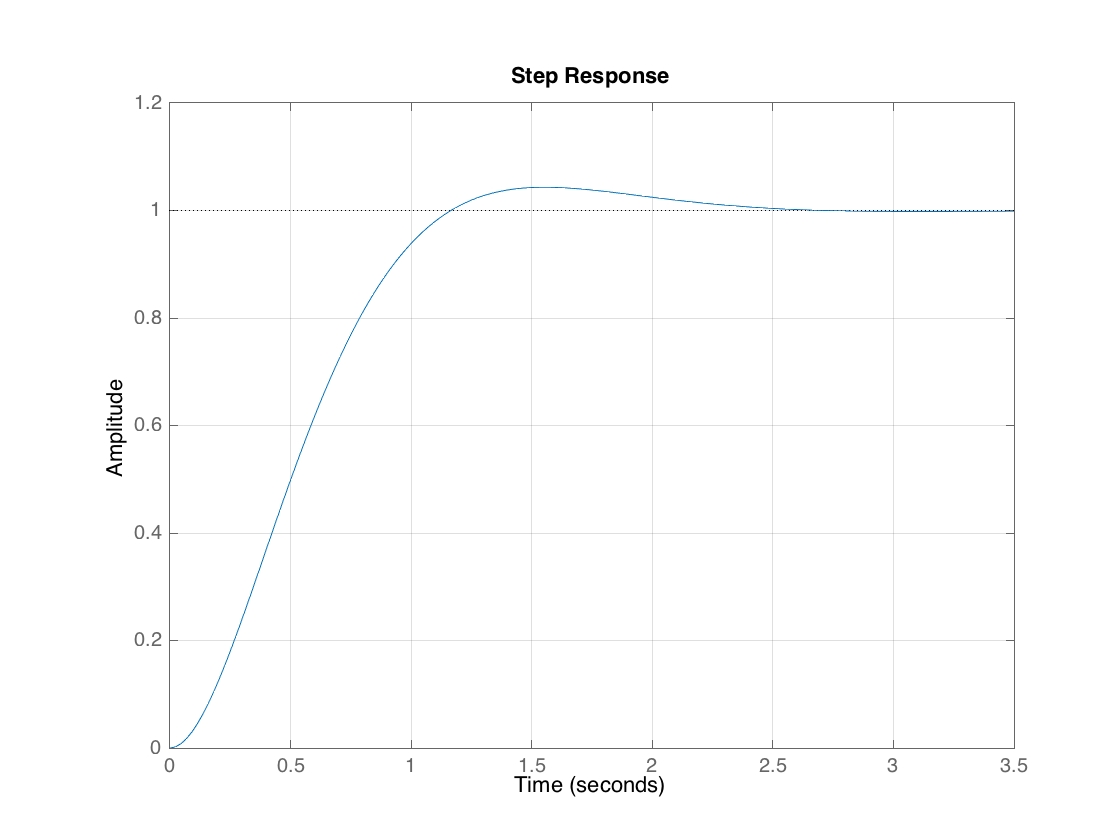
\includegraphics[scale = 0.3]{StepResponseFullOrderEst}
\caption{Step response of full-order estimator together with state feedback controller, rigid body model}
\label{StepResponseFullOrderEst}
\end{figure}

%Sinusoidal
\begin{figure}[!htbp]
\centering
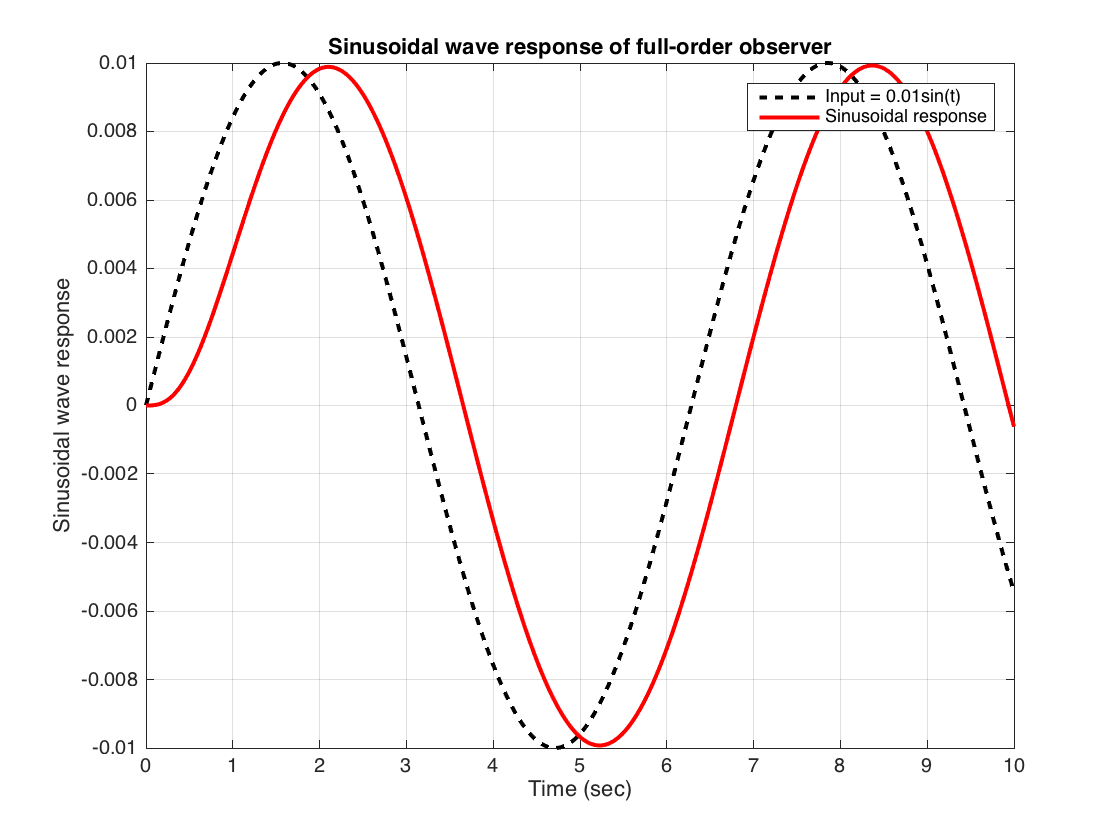
\includegraphics[scale = 0.3]{SinusoidalResponseFullOrderEst}
\caption{Sinusoidal wave response of full-order estimator together with state feedback controller, rigid body model}
\label{SinusoidalResponseFullOrderEst}
\end{figure}


% Flexible drive model
% Step response
\begin{figure}[!htbp]
\centering
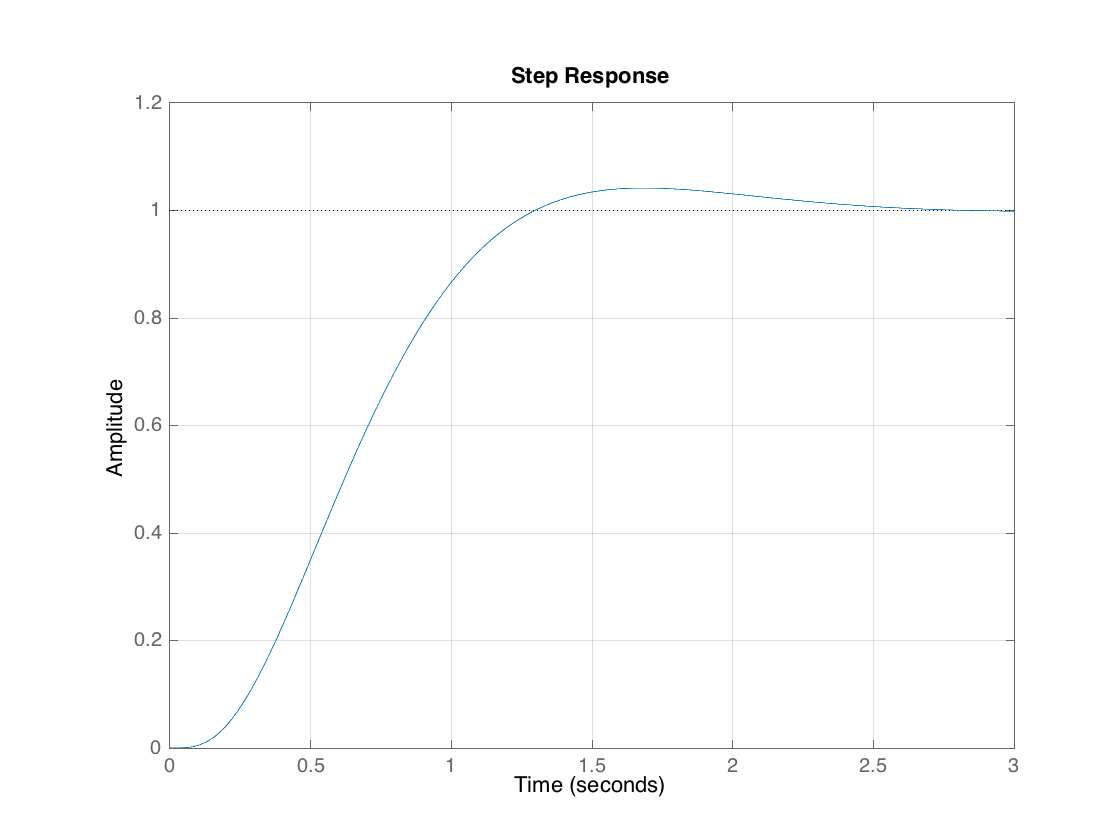
\includegraphics[scale = 0.3]{FlexibleStepResponseFullOrderEst}
\caption{Step response of full-order estimator together with state feedback controller, flexible drive model}
\label{FlexibleStepResponseFullOrderEst}
\end{figure}

%Sinusoidal
\begin{figure}[!htbp]
\centering
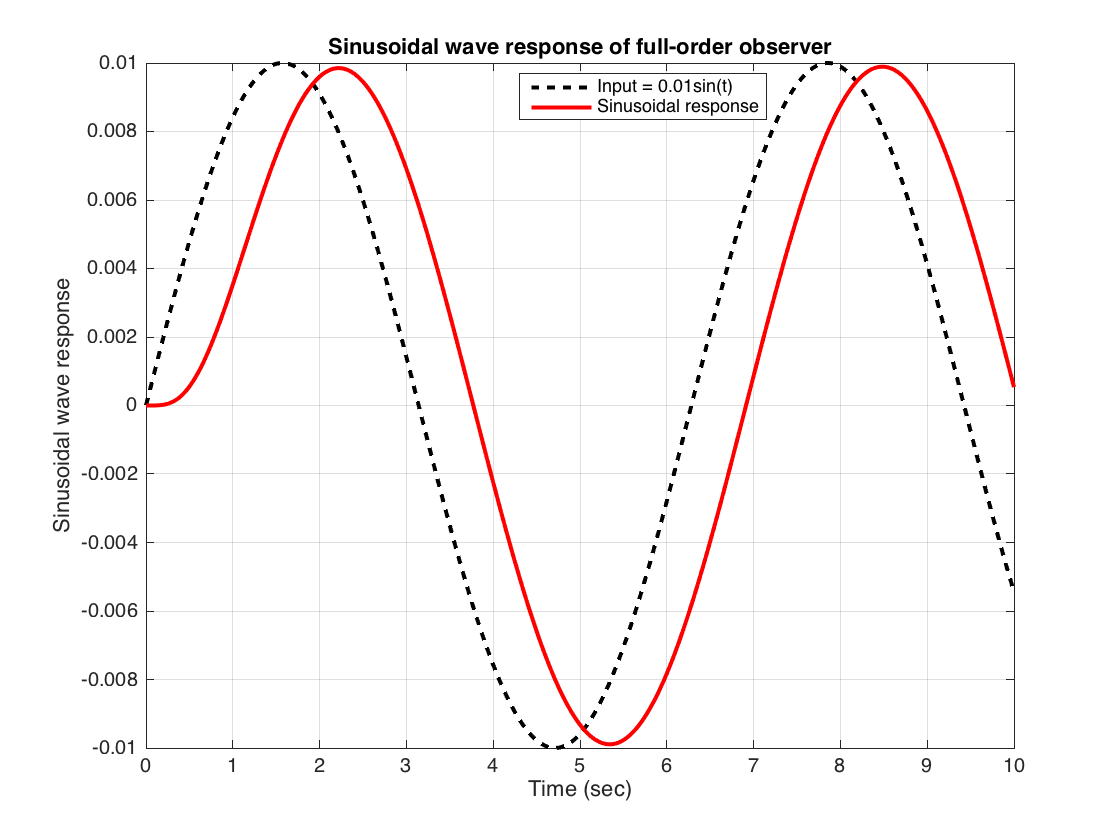
\includegraphics[scale = 0.3]{FlexibleSinusoidalResponseFullOrderEst}
\caption{Sinusoidal wave response of full-order estimator together with state feedback controller, flexible drive model}
\label{FlexibleSinusoidalResponseFullOrderEst}
\end{figure}

\newpage
% Reduced-order estimator
\subsection{Reduced-order observer}
\subsubsection{Rigid body model}
The reduced-order observer is reduced to a first-order system. We set the desired pole at $-15$ because it is five times away from the desired poles of full-order observer $-2.022\pm 2.0226i$. 

Then A can partitioned as $\begin{bmatrix} a_{11} &  A_{1e} \\ 
A_{e1}	&	A_{ee} \end{bmatrix}$, where $a_{11} =0$, $A_{1e} = 1$, $A_{e1} = 0$, and $A_{ee} = -1.782$.

Let $G_e = \begin{bmatrix} g \end{bmatrix}$. The desired characteristic polynomial is 

\begin{equation}\label{ReduEstPoly}
s+15
\end{equation}

\begin{equation}\label{findReduEstPoly}
det[sI - A_{ee} + G_e A_{1e}] = s+1.782+g
\end{equation}

Let equation~\ref{ReduEstPoly} = equation~\ref{findReduEstPoly}, then get g = 13.218.

\begin{equation}\label{ReduG4Rigid}
\mathbf{G} = \begin{bmatrix} 13.218	\end{bmatrix}
\end{equation}

\subsubsection{Flexible drive model}
\hspace{2.5ex} We used the same method as we did for rigid body model. We wrote the procedure in a m-file so that Matlab does the calculation. 

The output of Matlab is as followed.
\begin{verbatim}
>> L

L =

   1.0e+04 *

   -0.0484   -5.4633    0.0192    0.8874
\end{verbatim}

\begin{equation}\label{ReduG4flexible}
\mathbf{G} = 
\begin{bmatrix}
91.8729	\\	0.5842	\\	-7.5693
\end{bmatrix}
\end{equation}


\subsection{Step and sinusoidal response for reduced-order observer}

% Rigid body model
% Step response
\begin{figure}[!htbp]
\centering
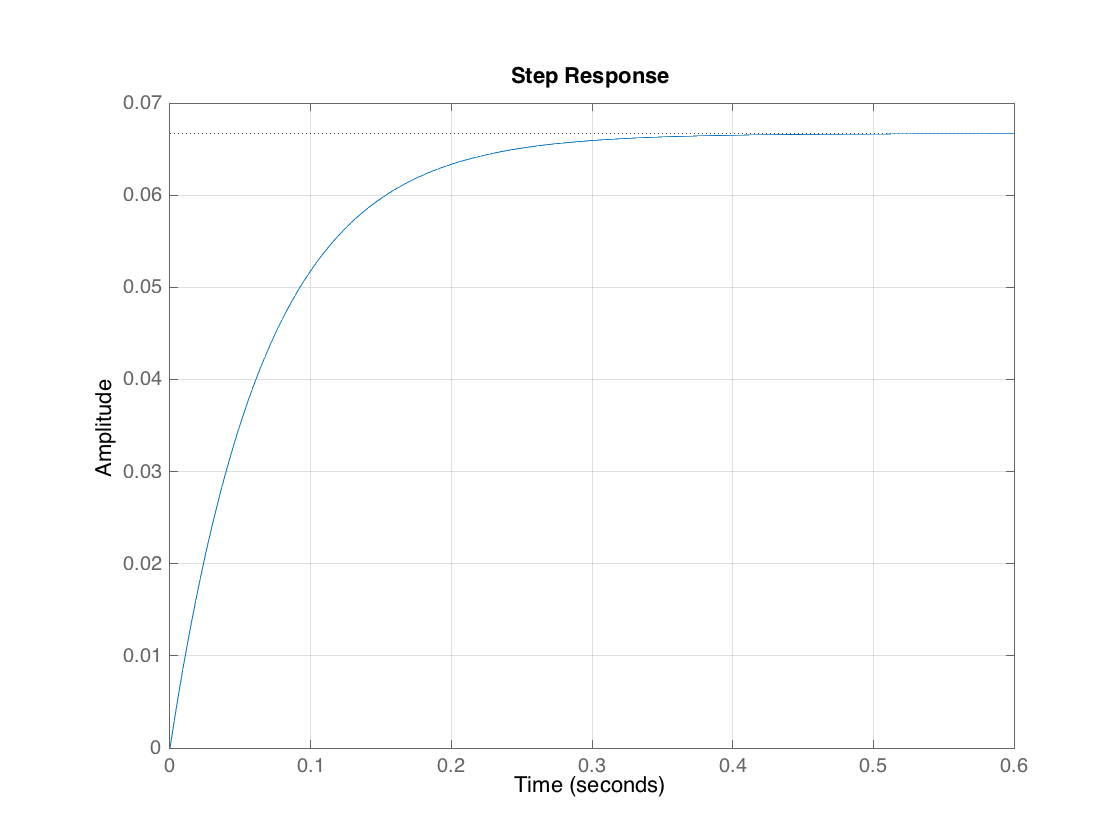
\includegraphics[scale = 0.3]{StepResponseReduOrderEst}
\caption{Step response of reduced-order estimator together with state feedback controller, rigid body model}
\label{StepResponseReduOrderEst}
\end{figure}

%Sinusoidal
\begin{figure}[!htbp]
\centering
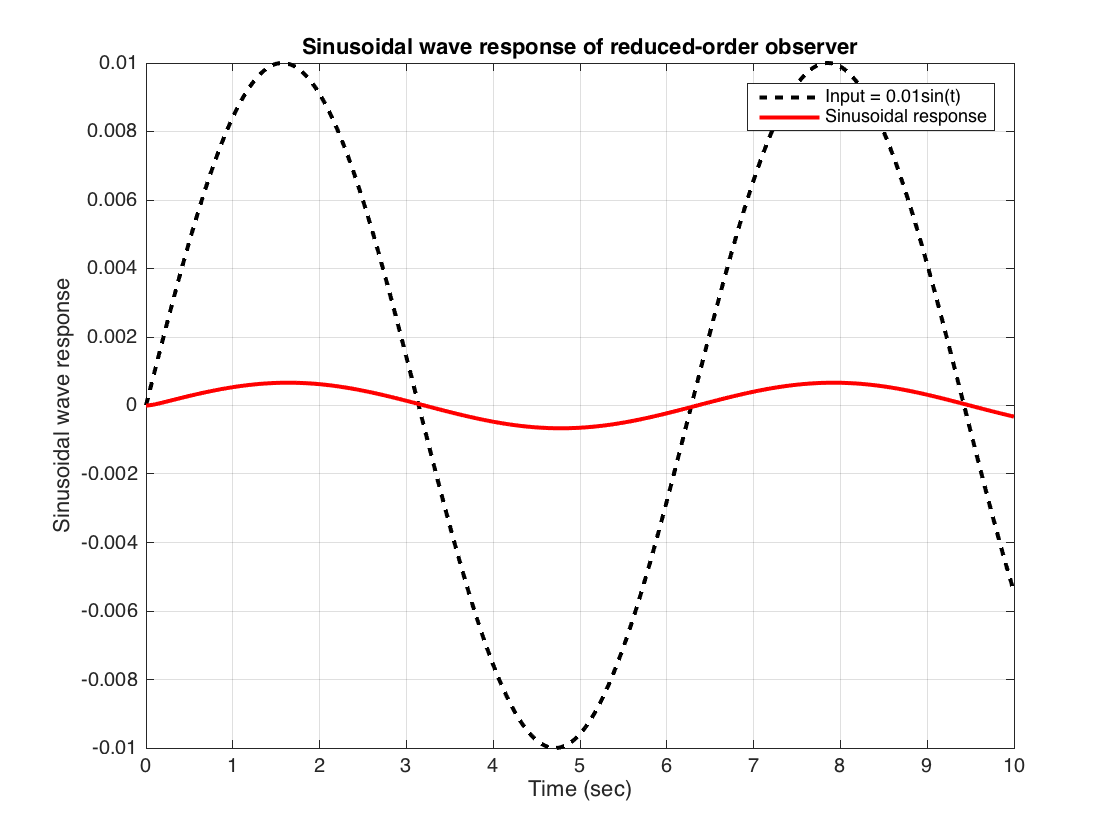
\includegraphics[scale = 0.3]{SinusoidalResponseReduOrderEst}
\caption{Sinusoidal wave response of reduced-order estimator together with state feedback controller, rigid body model}
\label{SinusoidalResponseReduOrderEst}
\end{figure}


% Flexible drive model
% Step response
\begin{figure}[!htbp]
\centering
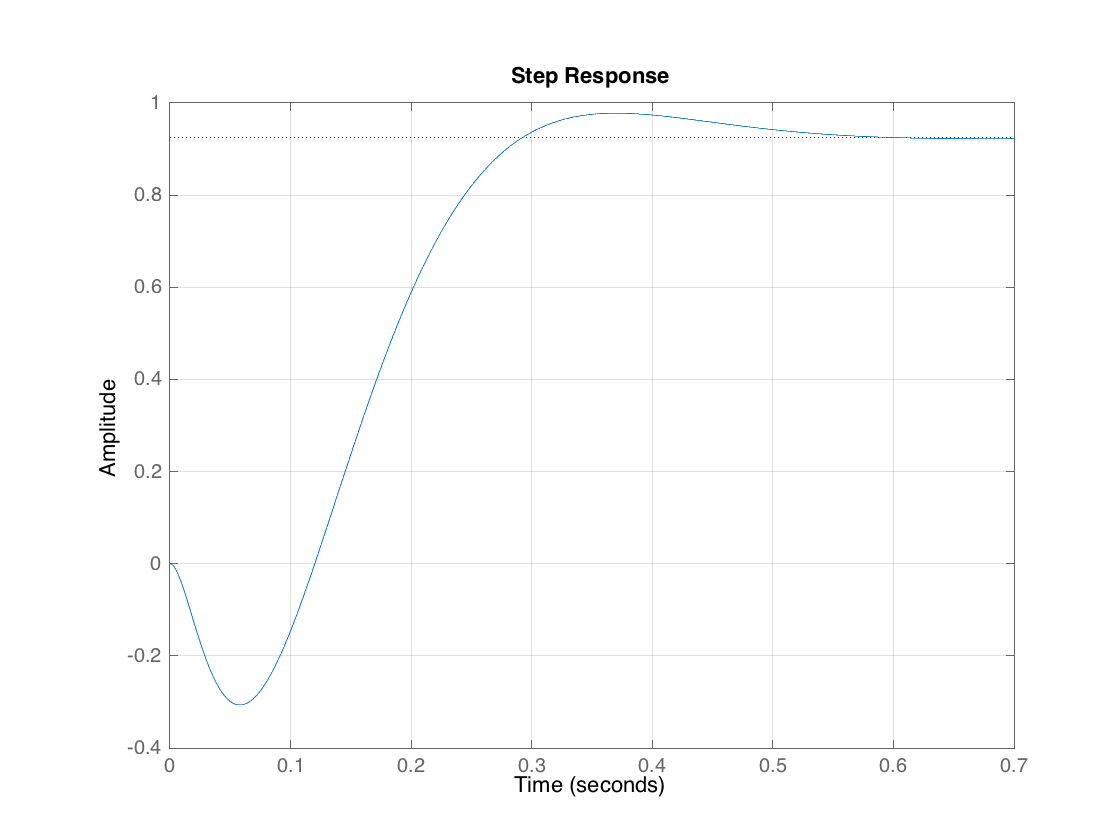
\includegraphics[scale = 0.3]{FlexibleStepResponseReduOrderEst}
\caption{Step response of reduced-order estimator together with state feedback controller, flexible drive model}
\label{FlexibleStepResponseReduOrderEst}
\end{figure}

%Sinusoidal
\begin{figure}[!htbp]
\centering
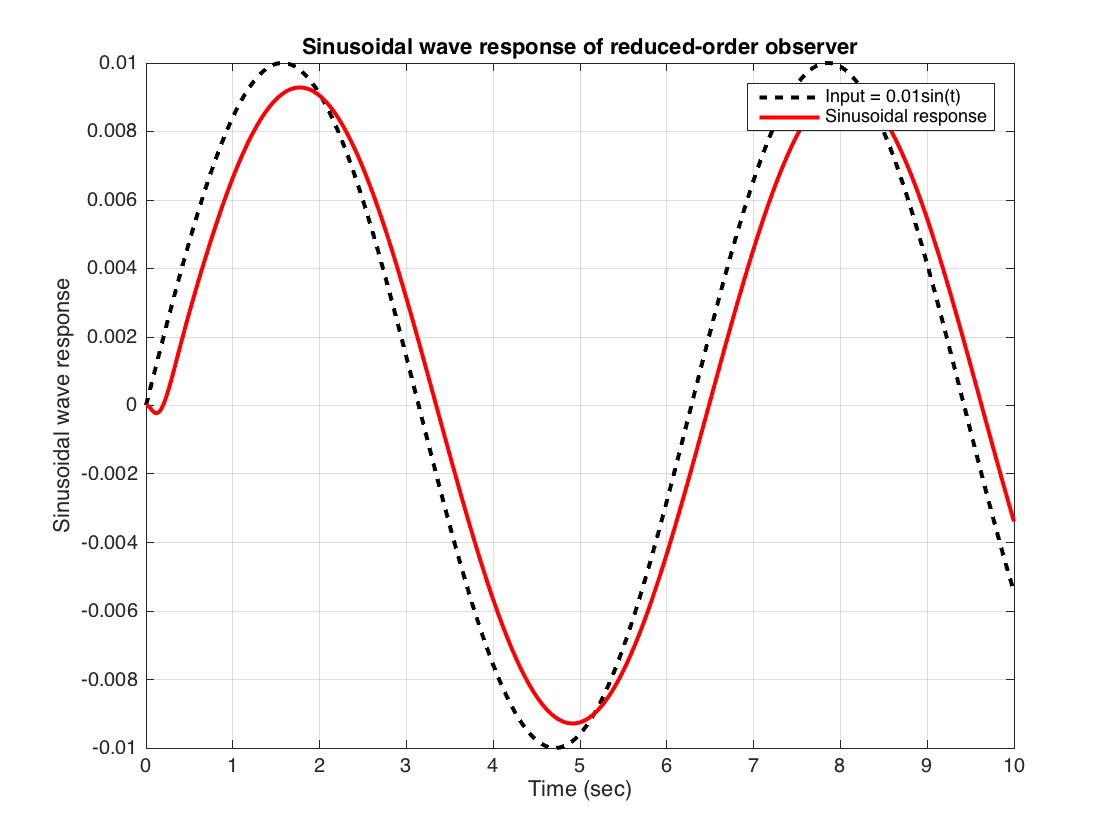
\includegraphics[scale = 0.3]{FlexibleSinusoidalResponseReduOrderEst}
\caption{Sinusoidal wave response of reduced-order estimator together with state feedback controller, flexible drive model}
\label{FlexibleSinusoidalResponseReduOrderEst}
\end{figure}


\newpage
%% Find the transfer function of the observer and controller. What type of controller do you get?
%==================================================Finished==============
\section{Find the transfer function of the observer and controller}
\hspace{2.5ex}
For simplicity, we only use rigid body model to find the transfer function of observer and controller by using the following formula: $G_{ec}(s) = K(sI  - A + BK + GC)^{-1} G$.

With $K= \begin{bmatrix} 0.0311 & 0.0086 \end{bmatrix}$ and $G = \begin{bmatrix} 18.4382 \\ 171.6332 \end{bmatrix}$, $N(s) = 2.0479s + 5.3378$.

$D(s) = (sI  - A + BK + GC) = s^2  + 22.484s + 254.37136$.

Therefore, $G_{ec} = \dfrac{2.0479s + 5.3378}{s^2  + 22.484s + 254.37136}$. Apparently, it is a lead-lag controller. 



%% Provide a comparative study between the classical control design advantages and disadvantages with that of the modern control theory design. ========================================
\section{Comparison between the classical and model control theory design}
\hspace{2.5ex}
Modern control theory uses time-domain state space representation while Classical control theory uses frequency domain analysis. Classical control theory put more emphasis on using methods such as root-locus and frequency response analysis. 
The advantage of using the root locus technique is that its easy to implement compared to other methods such as pole assignment, root locus also allows us to predict the performance of the whole system, and it provides a better way to indicate parameters\footnote{http://www.electrical4u.com/root-locus-technique-in-control-system-root-locus-plot/}.  Root loci also give good indication of transient response and explicitly show the locations of closed-loop poles\footnote{http://mocha-java.uccs.edu/ECE4510/ECE4510-Notes08.pdf}. 
However, frequency domain analysis requires transfer function of the plant to be known, it is also difficult to infer all performance values and to extract steady-state response\footnote{http://mocha-java.uccs.edu/ECE4510/ECE4510-Notes08.pdf}.

Meanwhile, modern control theory mainly uses pole assignment method augmented with observer, and optimal quadratic-loss control method. Some advantages of using methods such as pole assignment include ability to easily handle systems with multiple input and output. The model provides a time-domain solution, and the solution is the same for single first-order differential equation. In addition, state representation modelling is also very efficient and easy to compute for computer simulations.

However, pole assignment method requires the system to be controllable in order to be able to use it.



%% End of Content ========================================================




%% Appendix =============================================================
\newpage
\addappheadtotoc
\appendixpage
\begin{appendices}
\pagenumbering{Roman}
%% put appendices here

\section{Matlab code used for simulation -- plant.m}
\begin{verbatim}
% plant.m
% This is the script Calculates inertias and builds the rigid body or
% flexible plant models
% Yuan Sun
% 2015-11-20

clc
clear

%% ****  Input Parameters ****

%%
% Select output location, Out:
%
%        % "1" = Encoder #1; 
%        % "2" = Encoder #2
Out = 2;    % choose Encoder #2

%%
% Plant configuration, cofig:
%
%        % "1" = Drive disk only, (use only out = 1)
%        % "2" = Drive & load disk -- rigid drive train
%        % "3" = Drive & load disk -- flexixble drive belt

Config = 2; % choose flexible drive belt

%%
% Selec mass parameters
mwd = 0.8; %(mass of brass weights on drive disk)
rwd = 0.05; %(radius from center of plate on drive disk)
mwl = 2.0; %(mass of brass weight on load disk)
rwl = 0.1; %(radius from center of plate on load disk)

%Lower (Drive) Pully: Select (decomment) one of the following as
%appropriate:
npd = 18; Jpd = 0.000003;  %(18 tooth)
%npd = 24, Jpd = 0.000008;   %(24 tooth)
%npd = 36, Jpd = 0.000039;  %(36 tooth)
%npd = 72, Jpd = 0.00055;   %(72 tooth)

%Upper (Load) Pulley: Select (decomment) one of the followint as
%appropriate:
%npl = 18, Jpl = 0.000003;  %(18 tooth)
%npl = 24, Jpl = 0.000008;  %(24 tooth)
%npl = 36, Jpl = 0.000039;  %(36 tooth)
npl = 72; Jpl = 0.00055;    %(72 tooth)

%Default frict coeff's -- change if setup-specific measurements available
c1 = 0.004;  % if belt from drive to SR ass'y attached
%c1 = 0.002 % if belt from drive to SR ass'y not attached
c2 = 0.05;   % if belt from drive to SR ass'y attached
c12 = 0.017; % viscous coupling between drive & load

k = 8.45; % Torsional spring constant

khw = 5.81;  %(Hardware gain, assume kg=1, it will be corrected below if out = 2)


%% ****  Transfer Function and State Space Model  ****

%%
% Gear ratios

gr = 6 * npd / npl; %24;  % This is the value we found    % 6 * npd / npl; 
--> this is suggested by instructor  % gear ratio
grprime = npd / 12; %6; % This is the value we found  % npd / 12;
 --> This is suggested % drive to SR pulley gear ratio

%%
% First calculate known inertias
Jdd = 0.0004;         %0.000326; % 0.000400 is given by instructor's suggestion
Jdl = 0.0065;
Jpbl = 0.000031;    % Backlash mechanism
Jp = Jpd+Jpl+Jpbl;

%%
% Calculate Drive inertia

% initializing
rwdo = 0; 
rwlo = 0;

%%
% Find which size weight used, can use only 0, 2, or 4 weights
if mwd < 0.81
    if mwd < 0.39
        rwdo = 0.016; % (smaller brass weight used)
    end
end

if mwd < 2.1
    if mwd > 0.9
        rwdo = 0.025;   % (larger brass weight used)
    end
end
%%
% Caculate intertia about weights own cg.
Jwdo = (1 / 2) * mwd * rwdo^2;

%%
% Combine drive inertia:
Jd = Jdd + mwd * rwd^2 + Jwdo;

%%
% Calculate Load inertia
if mwl < 0.81
    if mwl > 0.39
        rwlo = 0.016; % (smaller brass weight used)
    end
end

if mwl < 2.1
    if mwl > 0.9
        rwlo = 0.025; % (larger brass weight used)
    end
end

%%
% Calculate inertia about weights own cg.
Jwlo = (1 / 2) * mwl * rwlo^2;

%%
%Combine load inertia
Jl = Jdl + mwl * rwl^2 + Jwlo;

%%
% Build transfer function and state space models
if Config == 1  % Drive disk only:
    %Transfer function:
    N = khw;
    D = [Jd c1 0];
    %State Space model:
    A1 = [0 1];
    A2 = [0 -c1/Jd];
    Aol = [A1; A2];
    B = [0 khw/Jd]';
    C = [1 0]; %Theta1 output
end

if Config == 2  % Drive & load disk -- rigid drive train
    if Out == 1 %Encode %1 output
        Jr = Jd + Jp * grprime^(-2) + Jl * gr^(-2);  %Reflected inertia at drive
        cr = c1 + c2 * gr^(-2);  %Relected damping to drive
        %Transfer Function:
        N = khw;
        D = [Jr cr 0];
        %State space model:
        A1 = [0 1];
        A2 = [0 -cr/Jr];
        Aol = [A1; A2];
        B = [0 khw/Jr]';
        C = [1 0];
    end
    if Out == 2 %Encode %2 output
        Jr = Jd * gr^2 + Jp * (gr / grprime)^2 + Jl; %Reflected inertia at load
        cr = c1 * gr^2 + c2;     %Reflected dampling at load
        %Transfer Function
        N = khw * gr;
        D = [Jr cr 0];
        %State space model:
        A1 = [0 1];
        A2 = [0 -cr/Jr];
        Aol = [A1; A2];
        B = [0 khw*gr/Jr]';
        C = [1 0];
    end
end

if Config == 3  %Drive & load disks -- flexible drive train
    Jdstr = Jd + Jp * grprime^(-2); %Pulley inertias combined with drive
    
    %Transfer Function
    %The following do not include the coupled damping c12
    N1 = khw * [Jl c2 k];
    N2 = khw * k / gr;
    D = [Jdstr*Jl (c2*Jdstr+c1*Jl) (k*(Jdstr+Jl/gr^2)+c1*c2) (k*(c1+c2/gr^2)) 0];
   
    %State space model
    A1 = [0 1 0 0];
    A3 = [0 0 0 1];
    %The following do not include the coupled damping c12
    A2 = [-k/Jdstr/gr^2 -c1/Jdstr k/Jdstr/gr 0];
    A4 = [k/Jl/gr 0 -k/Jl -c2/Jl];
    
    Aol = [A1; A2; A3; A4];
    B = [0 khw/Jdstr 0 0]';
    if Out == 1 %Encode %1 output
        C = [1 0 0 0];
    end
    if Out == 2 %Encode %2 output
        C = [0 0 1 0];
    end
end

% End of construct the plant 

%% 2. Construct transfer function
% Write transfer function directly
s = tf('s');

if Config == 1 || Config == 2
    num = N / D(1);
    den(2) = D(2) / D(1);
    den(3) = 0;
    den(1) = 1;
    H = tf(num, den);
end

if Config == 3
    num = N2 / D(1);
    den(2) = D(2) / D(1);
    den(3) = D(3) / D(1);
    den(4) = D(4) / D(1);
    den(1) = 1;
    den(5) = 0;
    H = tf(num, den);
end

% Write the system using A, B, C, and D
sys = ss(Aol, B, C, 0);



%% 3. Find Controllable, Observable, and Jordam Canonical Form
% Controllable and Observable form can be found by hand 
[Ac, Bc, Cc, Dc, P1] = canon(Aol, B, C, 0, 'companion'); % This is observable form

% Jorndan form
[V,J] = jordan(Aol);
[AJ, BJ, CJ, DJ, P2] = canon(Aol, B, C, 0);


%% 4. Find impulse response and step response
% Find close loop system

Hcl = 1/(1+sys); % or use command Hcl = feedback(sys, 1);


% % Impulse response
% 
% figure
% impulse(Hcl);
% grid;
% 
% % Step response
% 
% figure
% stepplot(Hcl);
% grid;

%% 5. Plot the Bode plot of the uncompensated system as well as root-locus of open loop system

% % Bode plot
% figure
% bode(sys);
% grid;
% 
% 
% % Root locus
% 
% figure
% rlocus(sys);
% grid;


%% 6. Design a lead-lag or a PID controller to meet certain design specifications (of your own choice). 
% Try to include both transient was well as steady state characteristics.
%
% Here is the design specification:
% $t_s$ <= 2s;
% P.O. < 5%; 
% $e_{ss}$ due to a step input is zero

%% 
%
% $$t_s \le 2 s $$  --> $\xi \omega \ge 2$ --> $\omega \ge \frac{2}{\xi} =2.86$; 
%
% $$P.O. \le 5 $$ --> $\theta < 45$ and $\xi = 0.707$; 
%
% $e_{ss}$ due to a step input is zero  --> put a 1/s in the forward path
%
% Design lead-lag compensator by using root-locus.
%
% The controller Gc is written as:

%%
% 
% $G_c = 0.012653 \frac{(1+0.56s)}{(1+0.23s)}$
%

if Config ==2
    Gc = 0.012134 * (1+0.56*s)/(1+0.25*s);
end

if Config == 3
    Gc = 0.012134 * (1+0.56*s)*(1+0.00091*s+(0.024*s)^2)/(1+0.25*s);
end

sys_controlled_op = Gc*H;
sys_controlled = Gc*sys/(1+Gc*sys);

%% 7. Obtain the step response, square wave and sinusoidal resposnes.

t = 0:0.01:10;

%% 
% Plot controlled step response

% figure
% step(sys_controlled);
% grid;

%%
% Square wave response;

[squareWave, tt] = gensig('square', 4, 10, 0.01);
% figure
% ysq = lsim(sys_controlled, squareWave, tt);
% plot(tt, squareWave, '--k', tt, ysq, '-r', 'LineWidth', 2);
% xlabel('Time (sec)');
% ylabel('Square wave response');
% legend('Input', 'Square wave response');
% grid;


%%
% Sinusoidal wave response;

u = 0.01*sin(t); % input

% figure
% ysq = lsim(sys_controlled, u, t);
% plot(t, u, '--k', t, ysq, '-r', 'LineWidth', 2);
% xlabel('Time (sec)');
% ylabel('Sinusoidal wave response');
% legend('Input = 0.01sin(t)', 'Sinusoidal response');
% grid;

%% 9. Design a full state feedback control to meet the design
 	specification indicated in (6)
% $\omega \ge 2.86$ 
%  and $\xi = 0.707$.
% 
% So characteristic equation is 
% $s^2 + 2\xi \omega s + \omega^2 = s^2 + 4.04404s + 8.1796$
% ** This is for second order system, so Config == 2

xi = 0.707;
omega = 2.86;


% Find pole

if Config == 2
    poles = [(-2*xi*omega+sqrt((2*xi*omega)^2-4*omega^2))/2 
    			(-2*xi*omega-sqrt((2*xi*omega)^2-4*omega^2))/2];
end

if Config ==3
    % To design a controller 4th order system, firstly satisfy the 
    % requirements of 2nd order system, then move other pole far way from 
    % jw axis to make them less dominent.
    % So take two poles same as 2nd order system, then 
    poles = [-20 -15 (-2*xi*omega+sqrt((2*xi*omega)^2-4*omega^2))/2 
    				(-2*xi*omega-sqrt((2*xi*omega)^2-4*omega^2))/2];
end

% Find K
    K = place(Aol, B, poles);
    Nbar = rscale(sys, K);
    
% Contructed controlled system by state feedback
    sys_cl = ss(Aol-B*K, B*Nbar, C, 0);

%% 10. Obtain the step, square wave and sinusoidal responses 
with arbitrary initial conditions and compare the results with those in 7.

%%
% Step response

% figure
% stepplot(sys_cl);
% grid;

%%
% Square wave response-- use lsim command

% figure
% ysq2 = lsim(sys_cl, squareWave, tt);
% plot(tt, squareWave, '--k', tt, ysq2, '-r', 'LineWidth', 2);
% xlabel('Time (sec)');
% ylabel('Square wave response');
% legend('Input', 'Square wave response');
% title('Square wave response using state feedback control');
% grid;
%%
% Sinusoidal wave response;
% 
% figure
% y1 = lsim(sys_cl, u, t);
% plot(t, u, '--k', t, y1, '-r', 'LineWidth', 2);
% xlabel('Time (sec)');
% ylabel('Sinusoidal wave response');
% legend('Input = 0.01sin(t)', 'Sinusoidal response');
% title('Sinusoidal wave response using state feedback control');
% grid;

%% 11. Design a full-order and a reduced-order observer 
and obtain step and sinusoidal response.

% --------------------
% Full-order observer -- with 5 times faster than designed controller

L = place(Aol', C', 5*poles);

At = [Aol-B*K B*K;
    zeros(size(Aol)) Aol-L'*C];
Bt = [B*Nbar; zeros(size(B))];
Ct = [C zeros(size(C))];

sys_est = ss(At, Bt, Ct, 0);

%% 
% Step response

% figure
% stepplot(sys_est); grid;

%%
% Sinusoidal wave response;

% figure
% y2 = lsim(sys_est, u, t);
% plot(t, u, '--k', t, y2, '-r', 'LineWidth', 2);
% xlabel('Time (sec)');
% ylabel('Sinusoidal wave response');
% legend('Input = 0.01sin(t)', 'Sinusoidal response');
% title('Sinusoidal wave response of full-order observer');
% grid;

% --------------------------
% Reduced-order observer

% Define requirements for reduced-order observer
% Define observer poles

if Config == 2
    % Reduce to 1st order system, with 3\tau < 2 --> \tau = 0.5 and \xi = 1
    % 5 times faster than controller.
    desiredPoles = -3*5;
    Aaa = [0];
    Aab = [1];
    Aba = [0];
    Abb = [-1.7820];
    
    L_redu = acker(Abb', Aab', desiredPoles')';
    A4reduObs = Abb - (L_redu * Aab);
    B4reduObs = eye(1);
    C4reduObs = eye(1);
end

if Config == 3
    % Reduce to 3rd order system, with desired poles of state feedback
    % controller except -20. 5 times faster than controller
    
    desiredPoles = 5*[-15 (-2*xi*omega+sqrt((2*xi*omega)^2-4*omega^2))/2 
    					(-2*xi*omega-sqrt((2*xi*omega)^2-4*omega^2))/2];
    Aaa = Aol(1);
    Aab = Aol(1, 2:4);
    Aba = Aol(2:4, 1);
    Abb = Aol(2:4, 2:4);
    
    L_redu = acker(Abb', Aab', desiredPoles')';
    A4reduObs = Abb - (L_redu * Aab);
    B4reduObs = B(2:4);
    C4reduObs = C(2:4);
end

%Reduced-order estimator
sys_reduEst = ss(A4reduObs, B4reduObs, C4reduObs, 0); 

%% 
% Step response
% 
% figure
% stepplot(sys_reduEst); grid;

%%
% Sinusoidal wave response;
% 
% figure
% y3 = lsim(sys_reduEst, u, t);
% plot(t, u, '--k', t, y3, '-r', 'LineWidth', 2);
% xlabel('Time (sec)');
% ylabel('Sinusoidal wave response');
% legend('Input = 0.01sin(t)', 'Sinusoidal response');
% title('Sinusoidal wave response of reduced-order observer');
% grid;


%% 12. Find the transfer function of the oberserver and controller. 

Gec_D = (s*eye(length(Aol)) - Aol + B*K + L'*C);  % D(s) of Gec

%End of Plant.m 
\end{verbatim}
\end{appendices}

\end{document}